% Options for packages loaded elsewhere
\PassOptionsToPackage{unicode}{hyperref}
\PassOptionsToPackage{hyphens}{url}
\PassOptionsToPackage{dvipsnames,svgnames,x11names}{xcolor}
%
\documentclass[
  letterpaper,
  DIV=11,
  numbers=noendperiod]{scrartcl}

\usepackage{amsmath,amssymb}
\usepackage{iftex}
\ifPDFTeX
  \usepackage[T1]{fontenc}
  \usepackage[utf8]{inputenc}
  \usepackage{textcomp} % provide euro and other symbols
\else % if luatex or xetex
  \usepackage{unicode-math}
  \defaultfontfeatures{Scale=MatchLowercase}
  \defaultfontfeatures[\rmfamily]{Ligatures=TeX,Scale=1}
\fi
\usepackage{lmodern}
\ifPDFTeX\else  
    % xetex/luatex font selection
\fi
% Use upquote if available, for straight quotes in verbatim environments
\IfFileExists{upquote.sty}{\usepackage{upquote}}{}
\IfFileExists{microtype.sty}{% use microtype if available
  \usepackage[]{microtype}
  \UseMicrotypeSet[protrusion]{basicmath} % disable protrusion for tt fonts
}{}
\makeatletter
\@ifundefined{KOMAClassName}{% if non-KOMA class
  \IfFileExists{parskip.sty}{%
    \usepackage{parskip}
  }{% else
    \setlength{\parindent}{0pt}
    \setlength{\parskip}{6pt plus 2pt minus 1pt}}
}{% if KOMA class
  \KOMAoptions{parskip=half}}
\makeatother
\usepackage{xcolor}
\setlength{\emergencystretch}{3em} % prevent overfull lines
\setcounter{secnumdepth}{-\maxdimen} % remove section numbering
% Make \paragraph and \subparagraph free-standing
\ifx\paragraph\undefined\else
  \let\oldparagraph\paragraph
  \renewcommand{\paragraph}[1]{\oldparagraph{#1}\mbox{}}
\fi
\ifx\subparagraph\undefined\else
  \let\oldsubparagraph\subparagraph
  \renewcommand{\subparagraph}[1]{\oldsubparagraph{#1}\mbox{}}
\fi

\usepackage{color}
\usepackage{fancyvrb}
\newcommand{\VerbBar}{|}
\newcommand{\VERB}{\Verb[commandchars=\\\{\}]}
\DefineVerbatimEnvironment{Highlighting}{Verbatim}{commandchars=\\\{\}}
% Add ',fontsize=\small' for more characters per line
\usepackage{framed}
\definecolor{shadecolor}{RGB}{241,243,245}
\newenvironment{Shaded}{\begin{snugshade}}{\end{snugshade}}
\newcommand{\AlertTok}[1]{\textcolor[rgb]{0.68,0.00,0.00}{#1}}
\newcommand{\AnnotationTok}[1]{\textcolor[rgb]{0.37,0.37,0.37}{#1}}
\newcommand{\AttributeTok}[1]{\textcolor[rgb]{0.40,0.45,0.13}{#1}}
\newcommand{\BaseNTok}[1]{\textcolor[rgb]{0.68,0.00,0.00}{#1}}
\newcommand{\BuiltInTok}[1]{\textcolor[rgb]{0.00,0.23,0.31}{#1}}
\newcommand{\CharTok}[1]{\textcolor[rgb]{0.13,0.47,0.30}{#1}}
\newcommand{\CommentTok}[1]{\textcolor[rgb]{0.37,0.37,0.37}{#1}}
\newcommand{\CommentVarTok}[1]{\textcolor[rgb]{0.37,0.37,0.37}{\textit{#1}}}
\newcommand{\ConstantTok}[1]{\textcolor[rgb]{0.56,0.35,0.01}{#1}}
\newcommand{\ControlFlowTok}[1]{\textcolor[rgb]{0.00,0.23,0.31}{#1}}
\newcommand{\DataTypeTok}[1]{\textcolor[rgb]{0.68,0.00,0.00}{#1}}
\newcommand{\DecValTok}[1]{\textcolor[rgb]{0.68,0.00,0.00}{#1}}
\newcommand{\DocumentationTok}[1]{\textcolor[rgb]{0.37,0.37,0.37}{\textit{#1}}}
\newcommand{\ErrorTok}[1]{\textcolor[rgb]{0.68,0.00,0.00}{#1}}
\newcommand{\ExtensionTok}[1]{\textcolor[rgb]{0.00,0.23,0.31}{#1}}
\newcommand{\FloatTok}[1]{\textcolor[rgb]{0.68,0.00,0.00}{#1}}
\newcommand{\FunctionTok}[1]{\textcolor[rgb]{0.28,0.35,0.67}{#1}}
\newcommand{\ImportTok}[1]{\textcolor[rgb]{0.00,0.46,0.62}{#1}}
\newcommand{\InformationTok}[1]{\textcolor[rgb]{0.37,0.37,0.37}{#1}}
\newcommand{\KeywordTok}[1]{\textcolor[rgb]{0.00,0.23,0.31}{#1}}
\newcommand{\NormalTok}[1]{\textcolor[rgb]{0.00,0.23,0.31}{#1}}
\newcommand{\OperatorTok}[1]{\textcolor[rgb]{0.37,0.37,0.37}{#1}}
\newcommand{\OtherTok}[1]{\textcolor[rgb]{0.00,0.23,0.31}{#1}}
\newcommand{\PreprocessorTok}[1]{\textcolor[rgb]{0.68,0.00,0.00}{#1}}
\newcommand{\RegionMarkerTok}[1]{\textcolor[rgb]{0.00,0.23,0.31}{#1}}
\newcommand{\SpecialCharTok}[1]{\textcolor[rgb]{0.37,0.37,0.37}{#1}}
\newcommand{\SpecialStringTok}[1]{\textcolor[rgb]{0.13,0.47,0.30}{#1}}
\newcommand{\StringTok}[1]{\textcolor[rgb]{0.13,0.47,0.30}{#1}}
\newcommand{\VariableTok}[1]{\textcolor[rgb]{0.07,0.07,0.07}{#1}}
\newcommand{\VerbatimStringTok}[1]{\textcolor[rgb]{0.13,0.47,0.30}{#1}}
\newcommand{\WarningTok}[1]{\textcolor[rgb]{0.37,0.37,0.37}{\textit{#1}}}

\providecommand{\tightlist}{%
  \setlength{\itemsep}{0pt}\setlength{\parskip}{0pt}}\usepackage{longtable,booktabs,array}
\usepackage{calc} % for calculating minipage widths
% Correct order of tables after \paragraph or \subparagraph
\usepackage{etoolbox}
\makeatletter
\patchcmd\longtable{\par}{\if@noskipsec\mbox{}\fi\par}{}{}
\makeatother
% Allow footnotes in longtable head/foot
\IfFileExists{footnotehyper.sty}{\usepackage{footnotehyper}}{\usepackage{footnote}}
\makesavenoteenv{longtable}
\usepackage{graphicx}
\makeatletter
\def\maxwidth{\ifdim\Gin@nat@width>\linewidth\linewidth\else\Gin@nat@width\fi}
\def\maxheight{\ifdim\Gin@nat@height>\textheight\textheight\else\Gin@nat@height\fi}
\makeatother
% Scale images if necessary, so that they will not overflow the page
% margins by default, and it is still possible to overwrite the defaults
% using explicit options in \includegraphics[width, height, ...]{}
\setkeys{Gin}{width=\maxwidth,height=\maxheight,keepaspectratio}
% Set default figure placement to htbp
\makeatletter
\def\fps@figure{htbp}
\makeatother

\KOMAoption{captions}{tableheading}
\makeatletter
\makeatother
\makeatletter
\makeatother
\makeatletter
\@ifpackageloaded{caption}{}{\usepackage{caption}}
\AtBeginDocument{%
\ifdefined\contentsname
  \renewcommand*\contentsname{Table of contents}
\else
  \newcommand\contentsname{Table of contents}
\fi
\ifdefined\listfigurename
  \renewcommand*\listfigurename{List of Figures}
\else
  \newcommand\listfigurename{List of Figures}
\fi
\ifdefined\listtablename
  \renewcommand*\listtablename{List of Tables}
\else
  \newcommand\listtablename{List of Tables}
\fi
\ifdefined\figurename
  \renewcommand*\figurename{Figure}
\else
  \newcommand\figurename{Figure}
\fi
\ifdefined\tablename
  \renewcommand*\tablename{Table}
\else
  \newcommand\tablename{Table}
\fi
}
\@ifpackageloaded{float}{}{\usepackage{float}}
\floatstyle{ruled}
\@ifundefined{c@chapter}{\newfloat{codelisting}{h}{lop}}{\newfloat{codelisting}{h}{lop}[chapter]}
\floatname{codelisting}{Listing}
\newcommand*\listoflistings{\listof{codelisting}{List of Listings}}
\makeatother
\makeatletter
\@ifpackageloaded{caption}{}{\usepackage{caption}}
\@ifpackageloaded{subcaption}{}{\usepackage{subcaption}}
\makeatother
\makeatletter
\@ifpackageloaded{tcolorbox}{}{\usepackage[skins,breakable]{tcolorbox}}
\makeatother
\makeatletter
\@ifundefined{shadecolor}{\definecolor{shadecolor}{rgb}{.97, .97, .97}}
\makeatother
\makeatletter
\makeatother
\makeatletter
\makeatother
\ifLuaTeX
  \usepackage{selnolig}  % disable illegal ligatures
\fi
\IfFileExists{bookmark.sty}{\usepackage{bookmark}}{\usepackage{hyperref}}
\IfFileExists{xurl.sty}{\usepackage{xurl}}{} % add URL line breaks if available
\urlstyle{same} % disable monospaced font for URLs
\hypersetup{
  pdftitle={Neiker},
  pdfauthor={Val F. Lanza},
  colorlinks=true,
  linkcolor={blue},
  filecolor={Maroon},
  citecolor={Blue},
  urlcolor={Blue},
  pdfcreator={LaTeX via pandoc}}

\title{Neiker}
\author{Val F. Lanza}
\date{}

\begin{document}
\maketitle
\ifdefined\Shaded\renewenvironment{Shaded}{\begin{tcolorbox}[boxrule=0pt, enhanced, breakable, frame hidden, interior hidden, sharp corners, borderline west={3pt}{0pt}{shadecolor}]}{\end{tcolorbox}}\fi

\begin{Shaded}
\begin{Highlighting}[]
\FunctionTok{library}\NormalTok{(tidyverse)}
\end{Highlighting}
\end{Shaded}

\begin{verbatim}
-- Attaching core tidyverse packages ------------------------ tidyverse 2.0.0 --
v dplyr     1.1.4     v readr     2.1.5
v forcats   1.0.0     v stringr   1.5.1
v ggplot2   3.5.1     v tibble    3.2.1
v lubridate 1.9.3     v tidyr     1.3.1
v purrr     1.0.2     
-- Conflicts ------------------------------------------ tidyverse_conflicts() --
x dplyr::filter() masks stats::filter()
x dplyr::lag()    masks stats::lag()
i Use the conflicted package (<http://conflicted.r-lib.org/>) to force all conflicts to become errors
\end{verbatim}

\begin{Shaded}
\begin{Highlighting}[]
\FunctionTok{library}\NormalTok{(vegan)}
\end{Highlighting}
\end{Shaded}

\begin{verbatim}
Cargando paquete requerido: permute
Cargando paquete requerido: lattice
This is vegan 2.6-4
\end{verbatim}

\begin{Shaded}
\begin{Highlighting}[]
\FunctionTok{library}\NormalTok{(ggsci)}
\FunctionTok{library}\NormalTok{(gamlss)}
\end{Highlighting}
\end{Shaded}

\begin{verbatim}
Cargando paquete requerido: splines
Cargando paquete requerido: gamlss.data

Adjuntando el paquete: 'gamlss.data'

The following object is masked from 'package:datasets':

    sleep

Cargando paquete requerido: gamlss.dist
Cargando paquete requerido: nlme

Adjuntando el paquete: 'nlme'

The following object is masked from 'package:dplyr':

    collapse

Cargando paquete requerido: parallel
 **********   GAMLSS Version 5.4-22  ********** 
For more on GAMLSS look at https://www.gamlss.com/
Type gamlssNews() to see new features/changes/bug fixes.
\end{verbatim}

\begin{Shaded}
\begin{Highlighting}[]
\FunctionTok{library}\NormalTok{(easystats)}
\end{Highlighting}
\end{Shaded}

\begin{verbatim}
# Attaching packages: easystats 0.7.1 (red = needs update)
√ bayestestR  0.13.2    √ correlation 0.8.4  
√ datawizard  0.10.0    x effectsize  0.8.7  
x insight     0.19.10   √ modelbased  0.8.7  
√ performance 0.11.0    x parameters  0.21.6 
√ report      0.5.8     √ see         0.8.4  

Restart the R-Session and update packages with `easystats::easystats_update()`.
\end{verbatim}

\begin{Shaded}
\begin{Highlighting}[]
\FunctionTok{library}\NormalTok{(ggstatsplot)}
\end{Highlighting}
\end{Shaded}

\begin{verbatim}
You can cite this package as:
     Patil, I. (2021). Visualizations with statistical details: The 'ggstatsplot' approach.
     Journal of Open Source Software, 6(61), 3167, doi:10.21105/joss.03167
\end{verbatim}

\begin{Shaded}
\begin{Highlighting}[]
\FunctionTok{library}\NormalTok{(dplyr)}
\FunctionTok{library}\NormalTok{(emmeans)}
\end{Highlighting}
\end{Shaded}

\hypertarget{loading-data}{%
\section{Loading data}\label{loading-data}}

\begin{Shaded}
\begin{Highlighting}[]
\CommentTok{\# files \textless{}{-} dir(".", pattern = "res")}
\CommentTok{\# }
\CommentTok{\# tabla \textless{}{-} data.frame()}
\CommentTok{\# }
\CommentTok{\# for (i in files)}
\CommentTok{\# \{}
\CommentTok{\#   tmp \textless{}{-} read\_tsv(i)}
\CommentTok{\#   sample \textless{}{-} gsub(".res","",i)}
\CommentTok{\#   tmp$Sample \textless{}{-} sample}
\CommentTok{\#   }
\CommentTok{\#   tabla \textless{}{-} bind\_rows(tabla,tmp)}
\CommentTok{\# \}}

\NormalTok{tabla }\OtherTok{\textless{}{-}} \FunctionTok{read\_csv}\NormalTok{(}\StringTok{"./miguel/neiker/tabla\_inicial.csv"}\NormalTok{)}
\end{Highlighting}
\end{Shaded}

\hypertarget{filter-and-transform}{%
\subsection{Filter and Transform}\label{filter-and-transform}}

\begin{Shaded}
\begin{Highlighting}[]
\NormalTok{tabla\_otu }\OtherTok{\textless{}{-}}\NormalTok{ tabla }\SpecialCharTok{\%\textgreater{}\%} 
  \FunctionTok{filter}\NormalTok{(template\_identity }\SpecialCharTok{\textgreater{}} \DecValTok{95} \SpecialCharTok{\&}\NormalTok{ template\_coverage }\SpecialCharTok{\textgreater{}} \DecValTok{95}\NormalTok{) }\SpecialCharTok{\%\textgreater{}\%} 
  \FunctionTok{group\_by}\NormalTok{(dataset,template) }\SpecialCharTok{\%\textgreater{}\%} 
  \FunctionTok{summarise}\NormalTok{(}\AttributeTok{depth =} \FunctionTok{max}\NormalTok{(depth), }
            \AttributeTok{template\_coverage =} \FunctionTok{max}\NormalTok{(template\_coverage), }
            \AttributeTok{template\_identity =} \FunctionTok{max}\NormalTok{(template\_identity)) }\SpecialCharTok{\%\textgreater{}\%} 
  \FunctionTok{ungroup}\NormalTok{() }\SpecialCharTok{\%\textgreater{}\%} 
\NormalTok{  dplyr}\SpecialCharTok{::}\FunctionTok{select}\NormalTok{(}\AttributeTok{Sample =}\NormalTok{ dataset,}\AttributeTok{gene =}\NormalTok{ template, depth) }\SpecialCharTok{\%\textgreater{}\%}
  \FunctionTok{group\_by}\NormalTok{(Sample,gene) }\SpecialCharTok{\%\textgreater{}\%} 
  \FunctionTok{summarise}\NormalTok{(}\AttributeTok{depth =} \FunctionTok{sum}\NormalTok{(depth)) }\SpecialCharTok{\%\textgreater{}\%} 
  \FunctionTok{pivot\_wider}\NormalTok{(}\AttributeTok{names\_from =}\NormalTok{ gene, }\AttributeTok{values\_from =}\NormalTok{ depth, }\AttributeTok{values\_fill =} \DecValTok{0}\NormalTok{)}
\end{Highlighting}
\end{Shaded}

\begin{verbatim}
`summarise()` has grouped output by 'dataset'. You can override using the
`.groups` argument.
`summarise()` has grouped output by 'Sample'. You can override using the
`.groups` argument.
\end{verbatim}

\hypertarget{load-metadata}{%
\subsection{Load Metadata}\label{load-metadata}}

\begin{Shaded}
\begin{Highlighting}[]
\NormalTok{metadata }\OtherTok{\textless{}{-}}\NormalTok{ readxl}\SpecialCharTok{::}\FunctionTok{read\_xlsx}\NormalTok{(}\StringTok{"Metadata.xlsx"}\NormalTok{)}

\NormalTok{metadata }\OtherTok{\textless{}{-}}\NormalTok{ metadata }\SpecialCharTok{\%\textgreater{}\%} 
  \FunctionTok{rename}\NormalTok{(}\AttributeTok{Sample =}\NormalTok{ Muestra) }\SpecialCharTok{\%\textgreater{}\%} 
  \FunctionTok{mutate}\NormalTok{(}\AttributeTok{toma =} \FunctionTok{as.character}\NormalTok{(}\StringTok{\textasciigrave{}}\AttributeTok{Fecha de muestreo}\StringTok{\textasciigrave{}}\NormalTok{))}
  
  
\NormalTok{full\_tabla }\OtherTok{\textless{}{-}}\NormalTok{ tabla }\SpecialCharTok{\%\textgreater{}\%} \FunctionTok{inner\_join}\NormalTok{(metadata }\SpecialCharTok{\%\textgreater{}\%} \FunctionTok{mutate}\NormalTok{(}\AttributeTok{dataset =} \FunctionTok{str\_c}\NormalTok{(}\StringTok{"Sample\_"}\NormalTok{,Sample)))}
\end{Highlighting}
\end{Shaded}

\begin{verbatim}
Joining with `by = join_by(dataset)`
\end{verbatim}

\begin{Shaded}
\begin{Highlighting}[]
\NormalTok{stats }\OtherTok{\textless{}{-}} \FunctionTok{read\_table}\NormalTok{(}\StringTok{"stats.tsv"}\NormalTok{)}
\end{Highlighting}
\end{Shaded}

\begin{verbatim}

-- Column specification --------------------------------------------------------
cols(
  file = col_character(),
  format = col_character(),
  type = col_character(),
  num_seqs = col_number(),
  sum_len = col_number(),
  min_len = col_double(),
  avg_len = col_double(),
  max_len = col_double()
)
\end{verbatim}

\begin{Shaded}
\begin{Highlighting}[]
\NormalTok{lista\_run }\OtherTok{\textless{}{-}} \FunctionTok{read\_tsv}\NormalTok{(}\StringTok{"lista.txt"}\NormalTok{, }\AttributeTok{col\_names =} \FunctionTok{c}\NormalTok{(}\StringTok{"Run"}\NormalTok{,}\StringTok{"file"}\NormalTok{)) }\SpecialCharTok{\%\textgreater{}\%} 
  \FunctionTok{mutate}\NormalTok{(}\AttributeTok{file =} \FunctionTok{gsub}\NormalTok{(}\StringTok{".fastq.gz"}\NormalTok{,}\StringTok{".clean.fastq.gz"}\NormalTok{,file))}
\end{Highlighting}
\end{Shaded}

\begin{verbatim}
Rows: 376 Columns: 2
-- Column specification --------------------------------------------------------
Delimiter: "\t"
chr (2): Run, file

i Use `spec()` to retrieve the full column specification for this data.
i Specify the column types or set `show_col_types = FALSE` to quiet this message.
\end{verbatim}

\begin{Shaded}
\begin{Highlighting}[]
\NormalTok{stats }\OtherTok{\textless{}{-}}\NormalTok{ stats }\SpecialCharTok{\%\textgreater{}\%} \FunctionTok{inner\_join}\NormalTok{(lista\_run) }\SpecialCharTok{\%\textgreater{}\%} 
  \FunctionTok{separate}\NormalTok{(file, }\FunctionTok{c}\NormalTok{(}\StringTok{"Pool"}\NormalTok{,}\StringTok{"Sample"}\NormalTok{,}\StringTok{"Pos"}\NormalTok{,}\StringTok{"line"}\NormalTok{,}\StringTok{"Read"}\NormalTok{,}\StringTok{"kk"}\NormalTok{), }\AttributeTok{sep =}\StringTok{"\_"}\NormalTok{) }\SpecialCharTok{\%\textgreater{}\%} 
  \FunctionTok{mutate}\NormalTok{(}\AttributeTok{Sample =} \FunctionTok{paste0}\NormalTok{(}\StringTok{"Sample\_"}\NormalTok{,Sample)) }\SpecialCharTok{\%\textgreater{}\%} 
  \FunctionTok{group\_by}\NormalTok{(Sample,Run) }\SpecialCharTok{\%\textgreater{}\%} \FunctionTok{summarise}\NormalTok{(}\AttributeTok{num\_seqs =} \FunctionTok{sum}\NormalTok{(num\_seqs), }\AttributeTok{sum\_len =} \FunctionTok{sum}\NormalTok{(sum\_len))}
\end{Highlighting}
\end{Shaded}

\begin{verbatim}
Joining with `by = join_by(file)`
`summarise()` has grouped output by 'Sample'. You can override using the
`.groups` argument.
\end{verbatim}

\begin{Shaded}
\begin{Highlighting}[]
\NormalTok{labels }\OtherTok{\textless{}{-}}\NormalTok{ full\_tabla }\SpecialCharTok{\%\textgreater{}\%} \FunctionTok{mutate}\NormalTok{(}\AttributeTok{label =} \FunctionTok{ifelse}\NormalTok{(database }\SpecialCharTok{==}\StringTok{"BAC"}\NormalTok{,Gene\_name,template)) }\SpecialCharTok{\%\textgreater{}\%}\NormalTok{ dplyr}\SpecialCharTok{::}\FunctionTok{select}\NormalTok{(template,label) }\SpecialCharTok{\%\textgreater{}\%} \FunctionTok{distinct}\NormalTok{()}



\NormalTok{full\_tabla }\SpecialCharTok{\%\textgreater{}\%} \FunctionTok{inner\_join}\NormalTok{(stats, }\AttributeTok{by =} \FunctionTok{c}\NormalTok{(}\StringTok{"dataset"} \OtherTok{=} \StringTok{"Sample"}\NormalTok{)) }\SpecialCharTok{\%\textgreater{}\%} 
  \FunctionTok{group\_by}\NormalTok{(Sample, num\_seqs, Run) }\SpecialCharTok{\%\textgreater{}\%} 
  \FunctionTok{summarise}\NormalTok{(}\AttributeTok{ToalDepth =} \FunctionTok{sum}\NormalTok{(depth)) }\SpecialCharTok{\%\textgreater{}\%} 
  \FunctionTok{ungroup}\NormalTok{() }\SpecialCharTok{\%\textgreater{}\%} 
  \FunctionTok{pivot\_longer}\NormalTok{(}\AttributeTok{names\_to =} \StringTok{"Type"}\NormalTok{, }\AttributeTok{values\_to =} \StringTok{"Value"}\NormalTok{, }\SpecialCharTok{{-}}\FunctionTok{c}\NormalTok{(Sample,Run)) }\SpecialCharTok{\%\textgreater{}\%} 
  \FunctionTok{ggplot}\NormalTok{(}\FunctionTok{aes}\NormalTok{(}\AttributeTok{x =}\NormalTok{ Sample, }\AttributeTok{y =}\NormalTok{ Value, }\AttributeTok{fill =}\NormalTok{Type)) }\SpecialCharTok{+} 
  \FunctionTok{geom\_col}\NormalTok{(}\AttributeTok{position =} \StringTok{"stack"}\NormalTok{) }\SpecialCharTok{+} 
  \FunctionTok{facet\_grid}\NormalTok{(Run }\SpecialCharTok{\textasciitilde{}}\NormalTok{., }\AttributeTok{scales =} \StringTok{"free\_y"}\NormalTok{) }\SpecialCharTok{+} 
  \FunctionTok{coord\_flip}\NormalTok{() }\SpecialCharTok{+}
  \FunctionTok{scale\_fill\_d3}\NormalTok{()}
\end{Highlighting}
\end{Shaded}

\begin{verbatim}
`summarise()` has grouped output by 'Sample', 'num_seqs'. You can override
using the `.groups` argument.
\end{verbatim}

\begin{figure}[H]

{\centering 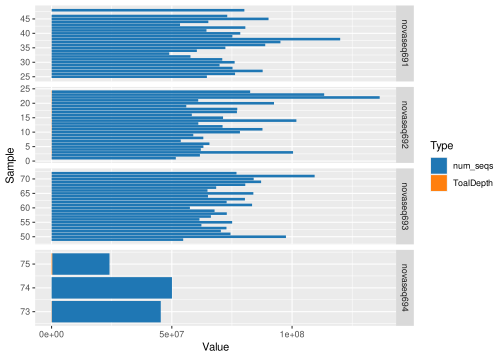
\includegraphics{InformeNeiker_files/figure-pdf/unnamed-chunk-4-1.pdf}

}

\end{figure}

\begin{Shaded}
\begin{Highlighting}[]
\NormalTok{full\_tabla }\SpecialCharTok{\%\textgreater{}\%} \FunctionTok{inner\_join}\NormalTok{(stats, }\AttributeTok{by =} \FunctionTok{c}\NormalTok{(}\StringTok{"dataset"} \OtherTok{=} \StringTok{"Sample"}\NormalTok{)) }\SpecialCharTok{\%\textgreater{}\%} 
  \FunctionTok{group\_by}\NormalTok{(Sample, }\AttributeTok{TotalReads =}\NormalTok{ num\_seqs, Run) }\SpecialCharTok{\%\textgreater{}\%} 
  \FunctionTok{summarise}\NormalTok{(}\AttributeTok{OnTarget =} \FunctionTok{sum}\NormalTok{(depth)) }\SpecialCharTok{\%\textgreater{}\%} 
  \FunctionTok{ungroup}\NormalTok{() }\SpecialCharTok{\%\textgreater{}\%} 
  \FunctionTok{pivot\_longer}\NormalTok{(}\AttributeTok{names\_to =} \StringTok{"Type"}\NormalTok{, }\AttributeTok{values\_to =} \StringTok{"Value"}\NormalTok{, }\SpecialCharTok{{-}}\FunctionTok{c}\NormalTok{(Sample,Run)) }\SpecialCharTok{\%\textgreater{}\%} 
  \CommentTok{\#filter(Run != "novaseq694") \%\textgreater{}\% }
  \FunctionTok{ggplot}\NormalTok{(}\FunctionTok{aes}\NormalTok{(}\AttributeTok{x =}\NormalTok{ Run, }\AttributeTok{y =}\NormalTok{ Value, }\AttributeTok{fill =}\NormalTok{Type)) }\SpecialCharTok{+} 
  \FunctionTok{geom\_boxplot}\NormalTok{(}\AttributeTok{alpha =} \FloatTok{0.8}\NormalTok{) }\SpecialCharTok{+} 
  \FunctionTok{geom\_dotplot}\NormalTok{(}\AttributeTok{binaxis =} \StringTok{"y"}\NormalTok{, }\AttributeTok{stackdir =} \StringTok{"center"}\NormalTok{,}\AttributeTok{shape =} \DecValTok{21}\NormalTok{) }\SpecialCharTok{+}
  \FunctionTok{facet\_wrap}\NormalTok{(Type }\SpecialCharTok{\textasciitilde{}}\NormalTok{., }\AttributeTok{scales =} \StringTok{"free"}\NormalTok{) }\SpecialCharTok{+} 
  \FunctionTok{scale\_fill\_d3}\NormalTok{() }\SpecialCharTok{+}
  \FunctionTok{theme\_light}\NormalTok{() }\SpecialCharTok{+}
  \FunctionTok{scale\_y\_log10}\NormalTok{() }\SpecialCharTok{+}
  \FunctionTok{theme}\NormalTok{(}\AttributeTok{axis.text =} \FunctionTok{element\_text}\NormalTok{(}\AttributeTok{angle =} \DecValTok{45}\NormalTok{, }\AttributeTok{hjust =} \DecValTok{1}\NormalTok{))}
\end{Highlighting}
\end{Shaded}

\begin{verbatim}
`summarise()` has grouped output by 'Sample', 'TotalReads'. You can override
using the `.groups` argument.
\end{verbatim}

\begin{verbatim}
Warning in geom_dotplot(binaxis = "y", stackdir = "center", shape = 21):
Ignoring unknown parameters: `shape`
\end{verbatim}

\begin{verbatim}
Bin width defaults to 1/30 of the range of the data. Pick better value with
`binwidth`.
\end{verbatim}

\begin{figure}[H]

{\centering \includegraphics{InformeNeiker_files/figure-pdf/unnamed-chunk-4-2.pdf}

}

\end{figure}

\begin{Shaded}
\begin{Highlighting}[]
\NormalTok{full\_tabla }\SpecialCharTok{\%\textgreater{}\%} 
  \FunctionTok{inner\_join}\NormalTok{(stats, }\AttributeTok{by =} \FunctionTok{c}\NormalTok{(}\StringTok{"dataset"} \OtherTok{=} \StringTok{"Sample"}\NormalTok{)) }\SpecialCharTok{\%\textgreater{}\%} 
  \FunctionTok{group\_by}\NormalTok{(Sample, }\AttributeTok{TotalReads =}\NormalTok{ num\_seqs, toma) }\SpecialCharTok{\%\textgreater{}\%} 
  \FunctionTok{summarise}\NormalTok{(}\AttributeTok{OnTarget =} \FunctionTok{sum}\NormalTok{(depth)) }\SpecialCharTok{\%\textgreater{}\%} 
  \FunctionTok{ungroup}\NormalTok{() }\SpecialCharTok{\%\textgreater{}\%} 
  \FunctionTok{pivot\_longer}\NormalTok{(}\AttributeTok{names\_to =} \StringTok{"Type"}\NormalTok{, }\AttributeTok{values\_to =} \StringTok{"Value"}\NormalTok{, }\SpecialCharTok{{-}}\FunctionTok{c}\NormalTok{(Sample,toma)) }\SpecialCharTok{\%\textgreater{}\%} 
  \CommentTok{\#filter(Run != "novaseq694") \%\textgreater{}\% }
  \FunctionTok{ggplot}\NormalTok{(}\FunctionTok{aes}\NormalTok{(}\AttributeTok{x =}\NormalTok{ toma, }\AttributeTok{y =}\NormalTok{ Value, }\AttributeTok{fill =}\NormalTok{Type)) }\SpecialCharTok{+} 
  \FunctionTok{geom\_boxplot}\NormalTok{(}\AttributeTok{alpha =} \FloatTok{0.8}\NormalTok{) }\SpecialCharTok{+} 
  \FunctionTok{geom\_dotplot}\NormalTok{(}\AttributeTok{binaxis =} \StringTok{"y"}\NormalTok{, }\AttributeTok{stackdir =} \StringTok{"center"}\NormalTok{,}\AttributeTok{shape =} \DecValTok{21}\NormalTok{) }\SpecialCharTok{+}
  \FunctionTok{facet\_wrap}\NormalTok{(Type }\SpecialCharTok{\textasciitilde{}}\NormalTok{., }\AttributeTok{scales =} \StringTok{"free"}\NormalTok{) }\SpecialCharTok{+} 
  \FunctionTok{scale\_fill\_d3}\NormalTok{() }\SpecialCharTok{+}
  \FunctionTok{theme\_light}\NormalTok{() }\SpecialCharTok{+}
  \FunctionTok{scale\_y\_log10}\NormalTok{() }\SpecialCharTok{+}
  \FunctionTok{theme}\NormalTok{(}\AttributeTok{axis.text =} \FunctionTok{element\_text}\NormalTok{(}\AttributeTok{angle =} \DecValTok{45}\NormalTok{, }\AttributeTok{hjust =} \DecValTok{1}\NormalTok{))}
\end{Highlighting}
\end{Shaded}

\begin{verbatim}
`summarise()` has grouped output by 'Sample', 'TotalReads'. You can override
using the `.groups` argument.
\end{verbatim}

\begin{verbatim}
Warning in geom_dotplot(binaxis = "y", stackdir = "center", shape = 21):
Ignoring unknown parameters: `shape`
\end{verbatim}

\begin{verbatim}
Bin width defaults to 1/30 of the range of the data. Pick better value with
`binwidth`.
\end{verbatim}

\begin{figure}[H]

{\centering \includegraphics{InformeNeiker_files/figure-pdf/unnamed-chunk-4-3.pdf}

}

\end{figure}

\hypertarget{quality-control}{%
\section{Quality Control}\label{quality-control}}

\begin{Shaded}
\begin{Highlighting}[]
\NormalTok{full\_tabla }\SpecialCharTok{\%\textgreater{}\%} \FunctionTok{filter}\NormalTok{(dataset }\SpecialCharTok{!=} \StringTok{"Sample\_75"}\NormalTok{) }\SpecialCharTok{\%\textgreater{}\%} 
  \FunctionTok{group\_by}\NormalTok{(dataset,}\StringTok{\textasciigrave{}}\AttributeTok{Cambio climático}\StringTok{\textasciigrave{}}\NormalTok{,Biocidas) }\SpecialCharTok{\%\textgreater{}\%} 
  \FunctionTok{summarise}\NormalTok{(}\AttributeTok{TotalCounts =} \FunctionTok{sum}\NormalTok{(depth)) }\SpecialCharTok{\%\textgreater{}\%} 
  \FunctionTok{ggplot}\NormalTok{(}\FunctionTok{aes}\NormalTok{(}\AttributeTok{x=}\NormalTok{ dataset, }\AttributeTok{y=}\NormalTok{TotalCounts, }\AttributeTok{fill =} \StringTok{\textasciigrave{}}\AttributeTok{Cambio climático}\StringTok{\textasciigrave{}}\NormalTok{)) }\SpecialCharTok{+} 
  \FunctionTok{geom\_col}\NormalTok{() }\SpecialCharTok{+}
  \FunctionTok{scale\_fill\_d3}\NormalTok{() }\SpecialCharTok{+}
  \FunctionTok{labs}\NormalTok{(}\AttributeTok{title =} \StringTok{"Total Depth Cambio Climatico"}\NormalTok{) }\SpecialCharTok{+}
  \FunctionTok{coord\_flip}\NormalTok{()}
\end{Highlighting}
\end{Shaded}

\begin{verbatim}
`summarise()` has grouped output by 'dataset', 'Cambio climático'. You can
override using the `.groups` argument.
\end{verbatim}

\begin{figure}[H]

{\centering 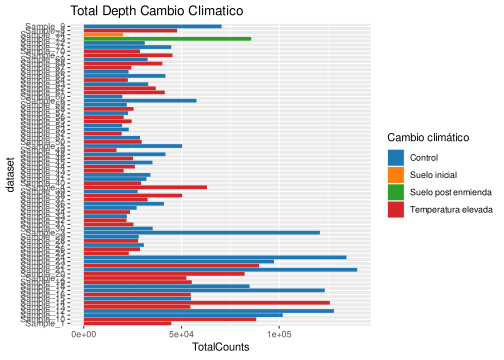
\includegraphics{InformeNeiker_files/figure-pdf/unnamed-chunk-5-1.pdf}

}

\end{figure}

\begin{Shaded}
\begin{Highlighting}[]
\NormalTok{full\_tabla }\SpecialCharTok{\%\textgreater{}\%} \FunctionTok{filter}\NormalTok{(dataset }\SpecialCharTok{!=} \StringTok{"Sample\_75"}\NormalTok{) }\SpecialCharTok{\%\textgreater{}\%} 
  \FunctionTok{group\_by}\NormalTok{(dataset,}\StringTok{\textasciigrave{}}\AttributeTok{Cambio climático}\StringTok{\textasciigrave{}}\NormalTok{,Biocidas) }\SpecialCharTok{\%\textgreater{}\%} 
  \FunctionTok{summarise}\NormalTok{(}\AttributeTok{TotalCounts =} \FunctionTok{sum}\NormalTok{(depth)) }\SpecialCharTok{\%\textgreater{}\%} 
  \FunctionTok{ggplot}\NormalTok{(}\FunctionTok{aes}\NormalTok{(}\AttributeTok{x=}\NormalTok{ dataset, }\AttributeTok{y=}\NormalTok{TotalCounts, }\AttributeTok{fill =}\NormalTok{ Biocidas)) }\SpecialCharTok{+} 
  \FunctionTok{geom\_col}\NormalTok{() }\SpecialCharTok{+}
  \FunctionTok{scale\_fill\_d3}\NormalTok{()}\SpecialCharTok{+}
  \FunctionTok{labs}\NormalTok{(}\AttributeTok{title =} \StringTok{"Total Depth Biocidas"}\NormalTok{) }\SpecialCharTok{+}
  \FunctionTok{coord\_flip}\NormalTok{()}
\end{Highlighting}
\end{Shaded}

\begin{verbatim}
`summarise()` has grouped output by 'dataset', 'Cambio climático'. You can
override using the `.groups` argument.
\end{verbatim}

\begin{figure}[H]

{\centering 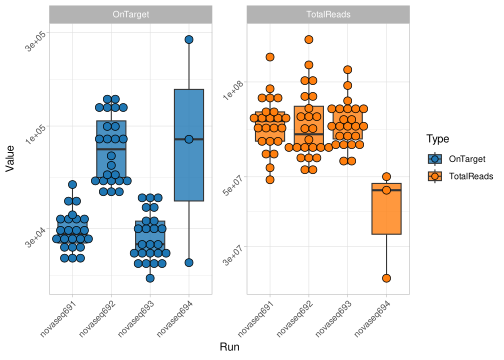
\includegraphics{InformeNeiker_files/figure-pdf/unnamed-chunk-5-2.pdf}

}

\end{figure}

\begin{Shaded}
\begin{Highlighting}[]
\NormalTok{full\_tabla }\SpecialCharTok{\%\textgreater{}\%} \FunctionTok{filter}\NormalTok{(dataset }\SpecialCharTok{!=} \StringTok{"Sample\_75"}\NormalTok{) }\SpecialCharTok{\%\textgreater{}\%} 
  \FunctionTok{group\_by}\NormalTok{(dataset,}\StringTok{\textasciigrave{}}\AttributeTok{Cambio climático}\StringTok{\textasciigrave{}}\NormalTok{,Biocidas) }\SpecialCharTok{\%\textgreater{}\%} 
  \FunctionTok{summarise}\NormalTok{(}\AttributeTok{TotalCounts =} \FunctionTok{sum}\NormalTok{(depth)) }\SpecialCharTok{\%\textgreater{}\%}
  \FunctionTok{ggplot}\NormalTok{(}\FunctionTok{aes}\NormalTok{(}\AttributeTok{x=} \StringTok{\textasciigrave{}}\AttributeTok{Cambio climático}\StringTok{\textasciigrave{}}\NormalTok{, }\AttributeTok{y=}\NormalTok{TotalCounts, }\AttributeTok{fill =} \StringTok{\textasciigrave{}}\AttributeTok{Cambio climático}\StringTok{\textasciigrave{}}\NormalTok{)) }\SpecialCharTok{+} 
  \FunctionTok{geom\_boxplot}\NormalTok{()}\SpecialCharTok{+}
  \FunctionTok{geom\_dotplot}\NormalTok{(}\AttributeTok{binaxis =} \StringTok{"y"}\NormalTok{, }\AttributeTok{stackdir =} \StringTok{"center"}\NormalTok{,}\AttributeTok{shape =} \DecValTok{21}\NormalTok{) }\SpecialCharTok{+}
  \FunctionTok{scale\_fill\_d3}\NormalTok{()}\SpecialCharTok{+}
  \FunctionTok{scale\_y\_log10}\NormalTok{()}\SpecialCharTok{+}
  \FunctionTok{labs}\NormalTok{(}\AttributeTok{title =} \StringTok{"Total Depth Cambio Climatico"}\NormalTok{)}
\end{Highlighting}
\end{Shaded}

\begin{verbatim}
`summarise()` has grouped output by 'dataset', 'Cambio climático'. You can
override using the `.groups` argument.
\end{verbatim}

\begin{verbatim}
Warning in geom_dotplot(binaxis = "y", stackdir = "center", shape = 21):
Ignoring unknown parameters: `shape`
\end{verbatim}

\begin{verbatim}
Bin width defaults to 1/30 of the range of the data. Pick better value with
`binwidth`.
\end{verbatim}

\begin{figure}[H]

{\centering 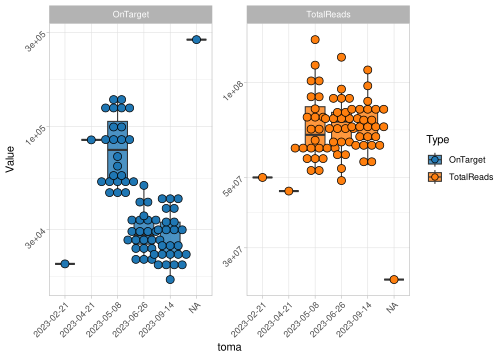
\includegraphics{InformeNeiker_files/figure-pdf/unnamed-chunk-5-3.pdf}

}

\end{figure}

\begin{Shaded}
\begin{Highlighting}[]
\NormalTok{full\_tabla }\SpecialCharTok{\%\textgreater{}\%} \FunctionTok{filter}\NormalTok{(dataset }\SpecialCharTok{!=} \StringTok{"Sample\_75"}\NormalTok{) }\SpecialCharTok{\%\textgreater{}\%} 
  \FunctionTok{group\_by}\NormalTok{(dataset,}\StringTok{\textasciigrave{}}\AttributeTok{Cambio climático}\StringTok{\textasciigrave{}}\NormalTok{,Biocidas) }\SpecialCharTok{\%\textgreater{}\%} 
  \FunctionTok{summarise}\NormalTok{(}\AttributeTok{TotalCounts =} \FunctionTok{sum}\NormalTok{(depth)) }\SpecialCharTok{\%\textgreater{}\%} 
  \FunctionTok{ggplot}\NormalTok{(}\FunctionTok{aes}\NormalTok{(}\AttributeTok{x=}\NormalTok{ Biocidas, }\AttributeTok{y=}\NormalTok{TotalCounts, }\AttributeTok{fill =}\NormalTok{ Biocidas)) }\SpecialCharTok{+} 
  \FunctionTok{geom\_boxplot}\NormalTok{()}\SpecialCharTok{+}
  \FunctionTok{geom\_dotplot}\NormalTok{(}\AttributeTok{binaxis =} \StringTok{"y"}\NormalTok{, }\AttributeTok{stackdir =} \StringTok{"center"}\NormalTok{,}\AttributeTok{shape =} \DecValTok{21}\NormalTok{) }\SpecialCharTok{+}
  \FunctionTok{scale\_fill\_d3}\NormalTok{()}\SpecialCharTok{+}
  \FunctionTok{scale\_y\_log10}\NormalTok{()}\SpecialCharTok{+}
  \FunctionTok{labs}\NormalTok{(}\AttributeTok{title =} \StringTok{"Total Depth Biocidas"}\NormalTok{)}
\end{Highlighting}
\end{Shaded}

\begin{verbatim}
`summarise()` has grouped output by 'dataset', 'Cambio climático'. You can
override using the `.groups` argument.
\end{verbatim}

\begin{verbatim}
Warning in geom_dotplot(binaxis = "y", stackdir = "center", shape = 21):
Ignoring unknown parameters: `shape`
\end{verbatim}

\begin{verbatim}
Bin width defaults to 1/30 of the range of the data. Pick better value with
`binwidth`.
\end{verbatim}

\begin{figure}[H]

{\centering \includegraphics{InformeNeiker_files/figure-pdf/unnamed-chunk-5-4.pdf}

}

\end{figure}

\begin{Shaded}
\begin{Highlighting}[]
\NormalTok{full\_tabla }\SpecialCharTok{\%\textgreater{}\%} \FunctionTok{filter}\NormalTok{(dataset }\SpecialCharTok{!=} \StringTok{"Sample\_75"}\NormalTok{) }\SpecialCharTok{\%\textgreater{}\%} 
  \FunctionTok{group\_by}\NormalTok{(dataset,toma) }\SpecialCharTok{\%\textgreater{}\%} 
  \FunctionTok{summarise}\NormalTok{(}\AttributeTok{TotalCounts =} \FunctionTok{sum}\NormalTok{(depth)) }\SpecialCharTok{\%\textgreater{}\%} 
  \FunctionTok{ggplot}\NormalTok{(}\FunctionTok{aes}\NormalTok{(}\AttributeTok{x=}\NormalTok{ toma, }\AttributeTok{y=}\NormalTok{TotalCounts, }\AttributeTok{fill =}\NormalTok{ toma)) }\SpecialCharTok{+} 
  \FunctionTok{geom\_boxplot}\NormalTok{()}\SpecialCharTok{+}
  \FunctionTok{geom\_dotplot}\NormalTok{(}\AttributeTok{binaxis =} \StringTok{"y"}\NormalTok{, }\AttributeTok{stackdir =} \StringTok{"center"}\NormalTok{,}\AttributeTok{shape =} \DecValTok{21}\NormalTok{) }\SpecialCharTok{+}
  \FunctionTok{scale\_fill\_d3}\NormalTok{()}\SpecialCharTok{+}
  \FunctionTok{scale\_y\_log10}\NormalTok{()}\SpecialCharTok{+}
  \FunctionTok{labs}\NormalTok{(}\AttributeTok{title =} \StringTok{"Total Depth toma"}\NormalTok{)}
\end{Highlighting}
\end{Shaded}

\begin{verbatim}
`summarise()` has grouped output by 'dataset'. You can override using the
`.groups` argument.
\end{verbatim}

\begin{verbatim}
Warning in geom_dotplot(binaxis = "y", stackdir = "center", shape = 21):
Ignoring unknown parameters: `shape`
\end{verbatim}

\begin{verbatim}
Bin width defaults to 1/30 of the range of the data. Pick better value with
`binwidth`.
\end{verbatim}

\begin{figure}[H]

{\centering \includegraphics{InformeNeiker_files/figure-pdf/unnamed-chunk-5-5.pdf}

}

\end{figure}

\begin{Shaded}
\begin{Highlighting}[]
\NormalTok{Validos }\OtherTok{\textless{}{-}}\NormalTok{ full\_tabla }\SpecialCharTok{\%\textgreater{}\%} 
  \FunctionTok{group\_by}\NormalTok{(dataset,template) }\SpecialCharTok{\%\textgreater{}\%} 
  \FunctionTok{summarise}\NormalTok{(}\AttributeTok{depth =} \FunctionTok{max}\NormalTok{(depth), }
            \AttributeTok{template\_coverage =} \FunctionTok{max}\NormalTok{(template\_coverage), }
            \AttributeTok{template\_identity =} \FunctionTok{max}\NormalTok{(template\_identity)) }\SpecialCharTok{\%\textgreater{}\%} 
  \FunctionTok{ungroup}\NormalTok{() }\SpecialCharTok{\%\textgreater{}\%} 
  \FunctionTok{group\_by}\NormalTok{(dataset) }\SpecialCharTok{\%\textgreater{}\%} 
  \FunctionTok{summarise}\NormalTok{(}\AttributeTok{TotalCounts =} \FunctionTok{sum}\NormalTok{(depth)) }\SpecialCharTok{\%\textgreater{}\%}
  \FunctionTok{filter}\NormalTok{(TotalCounts }\SpecialCharTok{\textgreater{}} \DecValTok{10000}\NormalTok{)}
\end{Highlighting}
\end{Shaded}

\begin{verbatim}
`summarise()` has grouped output by 'dataset'. You can override using the
`.groups` argument.
\end{verbatim}

\hypertarget{alpha-diversity}{%
\section{Alpha Diversity}\label{alpha-diversity}}

\begin{Shaded}
\begin{Highlighting}[]
\NormalTok{MinSampleSize }\OtherTok{\textless{}{-}}\NormalTok{ Validos }\SpecialCharTok{\%\textgreater{}\%} \FunctionTok{pull}\NormalTok{(TotalCounts) }\SpecialCharTok{\%\textgreater{}\%} \FunctionTok{min}\NormalTok{()}

\NormalTok{rare\_table }\OtherTok{\textless{}{-}}\NormalTok{ full\_tabla }\SpecialCharTok{\%\textgreater{}\%} 
  \FunctionTok{semi\_join}\NormalTok{(Validos) }\SpecialCharTok{\%\textgreater{}\%} 
  \FunctionTok{group\_by}\NormalTok{(dataset,template) }\SpecialCharTok{\%\textgreater{}\%} 
  \FunctionTok{summarise}\NormalTok{(}\AttributeTok{depth =} \FunctionTok{max}\NormalTok{(depth), }
            \AttributeTok{template\_coverage =} \FunctionTok{max}\NormalTok{(template\_coverage), }
            \AttributeTok{template\_identity =} \FunctionTok{max}\NormalTok{(template\_identity)) }\SpecialCharTok{\%\textgreater{}\%} 
  \FunctionTok{ungroup}\NormalTok{() }\SpecialCharTok{\%\textgreater{}\%} 
  \FunctionTok{filter}\NormalTok{(template\_coverage }\SpecialCharTok{\textgreater{}} \DecValTok{85}\NormalTok{, template\_identity }\SpecialCharTok{\textgreater{}} \DecValTok{85}\NormalTok{) }\SpecialCharTok{\%\textgreater{}\%} 
\NormalTok{  dplyr}\SpecialCharTok{::}\FunctionTok{select}\NormalTok{(dataset, template, depth) }\SpecialCharTok{\%\textgreater{}\%} 
  \FunctionTok{mutate}\NormalTok{(}\AttributeTok{depth =} \FunctionTok{round}\NormalTok{(depth)) }\SpecialCharTok{\%\textgreater{}\%} 
  \FunctionTok{pivot\_wider}\NormalTok{(}\AttributeTok{names\_from =}\NormalTok{ template, }\AttributeTok{values\_from =}\NormalTok{ depth, }\AttributeTok{values\_fill =}\DecValTok{0}\NormalTok{) }\SpecialCharTok{\%\textgreater{}\%} 
  \FunctionTok{column\_to\_rownames}\NormalTok{(}\StringTok{"dataset"}\NormalTok{) }\SpecialCharTok{\%\textgreater{}\%} 
  \FunctionTok{as.matrix}\NormalTok{() }\SpecialCharTok{\%\textgreater{}\%} 
  \FunctionTok{rrarefy}\NormalTok{( }\AttributeTok{sample =}\NormalTok{ MinSampleSize)}
\end{Highlighting}
\end{Shaded}

\begin{verbatim}
Joining with `by = join_by(dataset)`
`summarise()` has grouped output by 'dataset'. You can override using the
`.groups` argument.
\end{verbatim}

\begin{verbatim}
Warning in rrarefy(., sample = MinSampleSize): some row sums < 'sample' and are
not rarefied
\end{verbatim}

\begin{Shaded}
\begin{Highlighting}[]
\NormalTok{Div }\OtherTok{\textless{}{-}} \FunctionTok{inner\_join}\NormalTok{(}
  \FunctionTok{data.frame}\NormalTok{(}\AttributeTok{Simpson =} \FunctionTok{diversity}\NormalTok{(rare\_table, }\AttributeTok{index =} \StringTok{"simpson"}\NormalTok{),}
            \AttributeTok{Shannon =} \FunctionTok{diversity}\NormalTok{(rare\_table, }\AttributeTok{index =} \StringTok{"shannon"}\NormalTok{)) }\SpecialCharTok{\%\textgreater{}\%} 
    \FunctionTok{rownames\_to\_column}\NormalTok{(}\StringTok{"Sample"}\NormalTok{),}
        \FunctionTok{estimateR}\NormalTok{(rare\_table) }\SpecialCharTok{\%\textgreater{}\%} 
    \FunctionTok{t}\NormalTok{() }\SpecialCharTok{\%\textgreater{}\%}
    \FunctionTok{as.data.frame}\NormalTok{() }\SpecialCharTok{\%\textgreater{}\%}  
    \FunctionTok{rownames\_to\_column}\NormalTok{(}\StringTok{"Sample"}\NormalTok{))}
\end{Highlighting}
\end{Shaded}

\begin{verbatim}
Joining with `by = join_by(Sample)`
\end{verbatim}

\begin{Shaded}
\begin{Highlighting}[]
\NormalTok{Div }\SpecialCharTok{\%\textgreater{}\%} 
  \FunctionTok{pivot\_longer}\NormalTok{(}\AttributeTok{names\_to =} \StringTok{"Index"}\NormalTok{, }\AttributeTok{values\_to =} \StringTok{"Value"}\NormalTok{, }\SpecialCharTok{{-}}\NormalTok{Sample) }\SpecialCharTok{\%\textgreater{}\%} 
  \FunctionTok{inner\_join}\NormalTok{(metadata }\SpecialCharTok{\%\textgreater{}\%} 
               \FunctionTok{mutate}\NormalTok{(}\AttributeTok{Sample =} \FunctionTok{str\_c}\NormalTok{(}\StringTok{"Sample\_"}\NormalTok{,Sample))) }\SpecialCharTok{\%\textgreater{}\%} 
  \FunctionTok{filter}\NormalTok{(}\StringTok{\textasciigrave{}}\AttributeTok{Cambio climático}\StringTok{\textasciigrave{}} \SpecialCharTok{==} \StringTok{"Control"} \SpecialCharTok{|} \StringTok{\textasciigrave{}}\AttributeTok{Cambio climático}\StringTok{\textasciigrave{}} \SpecialCharTok{==} \StringTok{"Temperatura elevada"}\NormalTok{) }\SpecialCharTok{\%\textgreater{}\%} 
  \FunctionTok{ggplot}\NormalTok{(}\FunctionTok{aes}\NormalTok{(}\AttributeTok{x =} \StringTok{\textasciigrave{}}\AttributeTok{Cambio climático}\StringTok{\textasciigrave{}}\NormalTok{, }\AttributeTok{y =}\NormalTok{ Value, }\AttributeTok{fill =} \StringTok{\textasciigrave{}}\AttributeTok{Cambio climático}\StringTok{\textasciigrave{}}\NormalTok{)) }\SpecialCharTok{+} 
  \FunctionTok{geom\_boxplot}\NormalTok{() }\SpecialCharTok{+} 
  \FunctionTok{geom\_dotplot}\NormalTok{(}\AttributeTok{binaxis =} \StringTok{"y"}\NormalTok{, }\AttributeTok{stackdir =} \StringTok{"center"}\NormalTok{,}\AttributeTok{shape =} \DecValTok{21}\NormalTok{) }\SpecialCharTok{+}
  \FunctionTok{facet\_wrap}\NormalTok{(}\SpecialCharTok{\textasciitilde{}}\NormalTok{Index, }\AttributeTok{scales =} \StringTok{"free"}\NormalTok{) }\SpecialCharTok{+}
  \FunctionTok{scale\_fill\_d3}\NormalTok{() }\SpecialCharTok{+} 
  \FunctionTok{theme\_light}\NormalTok{() }\SpecialCharTok{+} \FunctionTok{coord\_flip}\NormalTok{()}
\end{Highlighting}
\end{Shaded}

\begin{verbatim}
Joining with `by = join_by(Sample)`
\end{verbatim}

\begin{verbatim}
Warning in geom_dotplot(binaxis = "y", stackdir = "center", shape = 21):
Ignoring unknown parameters: `shape`
\end{verbatim}

\begin{verbatim}
Bin width defaults to 1/30 of the range of the data. Pick better value with
`binwidth`.
\end{verbatim}

\begin{figure}[H]

{\centering 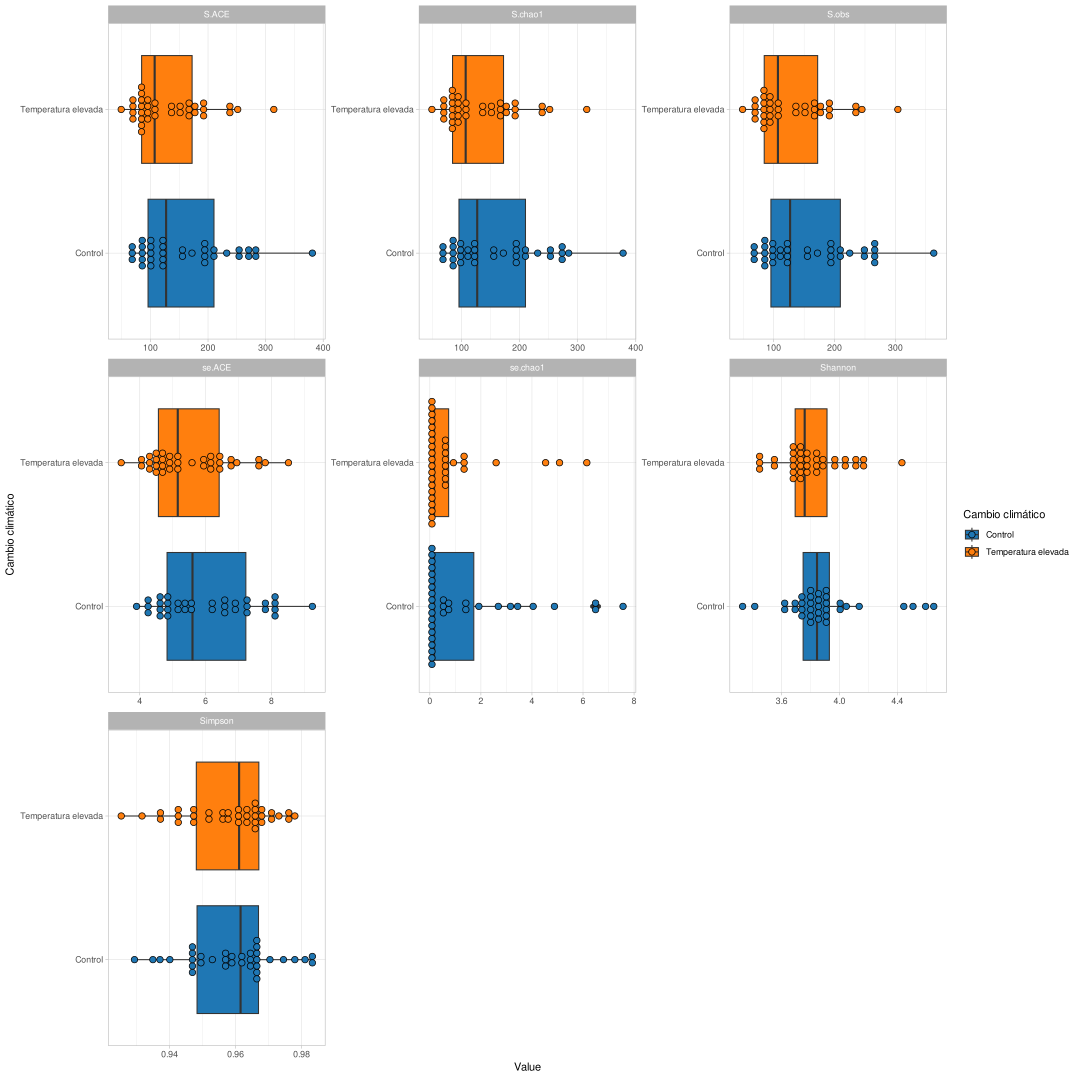
\includegraphics{InformeNeiker_files/figure-pdf/unnamed-chunk-7-1.pdf}

}

\end{figure}

\begin{Shaded}
\begin{Highlighting}[]
\NormalTok{Div }\SpecialCharTok{\%\textgreater{}\%} 
  \FunctionTok{pivot\_longer}\NormalTok{(}\AttributeTok{names\_to =} \StringTok{"Index"}\NormalTok{, }\AttributeTok{values\_to =} \StringTok{"Value"}\NormalTok{, }\SpecialCharTok{{-}}\NormalTok{Sample) }\SpecialCharTok{\%\textgreater{}\%} 
  \FunctionTok{inner\_join}\NormalTok{(metadata }\SpecialCharTok{\%\textgreater{}\%} 
               \FunctionTok{mutate}\NormalTok{(}\AttributeTok{Sample =} \FunctionTok{str\_c}\NormalTok{(}\StringTok{"Sample\_"}\NormalTok{,Sample))) }\SpecialCharTok{\%\textgreater{}\%} 
  \FunctionTok{filter}\NormalTok{(}\StringTok{\textasciigrave{}}\AttributeTok{Cambio climático}\StringTok{\textasciigrave{}} \SpecialCharTok{==} \StringTok{"Control"} \SpecialCharTok{|} \StringTok{\textasciigrave{}}\AttributeTok{Cambio climático}\StringTok{\textasciigrave{}} \SpecialCharTok{==} \StringTok{"Temperatura elevada"}\NormalTok{) }\SpecialCharTok{\%\textgreater{}\%} 
  \FunctionTok{ggplot}\NormalTok{(}\FunctionTok{aes}\NormalTok{(}\AttributeTok{x =}\NormalTok{ Biocidas, }\AttributeTok{y =}\NormalTok{ Value, }\AttributeTok{fill =}\NormalTok{ Biocidas)) }\SpecialCharTok{+} 
  \FunctionTok{geom\_boxplot}\NormalTok{() }\SpecialCharTok{+} 
  \FunctionTok{geom\_dotplot}\NormalTok{(}\AttributeTok{binaxis =} \StringTok{"y"}\NormalTok{, }\AttributeTok{stackdir =} \StringTok{"center"}\NormalTok{,}\AttributeTok{shape =} \DecValTok{21}\NormalTok{) }\SpecialCharTok{+}
  \FunctionTok{facet\_wrap}\NormalTok{(}\SpecialCharTok{\textasciitilde{}}\NormalTok{Index, }\AttributeTok{scales =} \StringTok{"free"}\NormalTok{) }\SpecialCharTok{+}
  \FunctionTok{scale\_fill\_d3}\NormalTok{() }\SpecialCharTok{+} 
  \FunctionTok{theme\_light}\NormalTok{() }\SpecialCharTok{+} \FunctionTok{coord\_flip}\NormalTok{()}
\end{Highlighting}
\end{Shaded}

\begin{verbatim}
Joining with `by = join_by(Sample)`
\end{verbatim}

\begin{verbatim}
Warning in geom_dotplot(binaxis = "y", stackdir = "center", shape = 21):
Ignoring unknown parameters: `shape`
\end{verbatim}

\begin{verbatim}
Bin width defaults to 1/30 of the range of the data. Pick better value with
`binwidth`.
\end{verbatim}

\begin{figure}[H]

{\centering 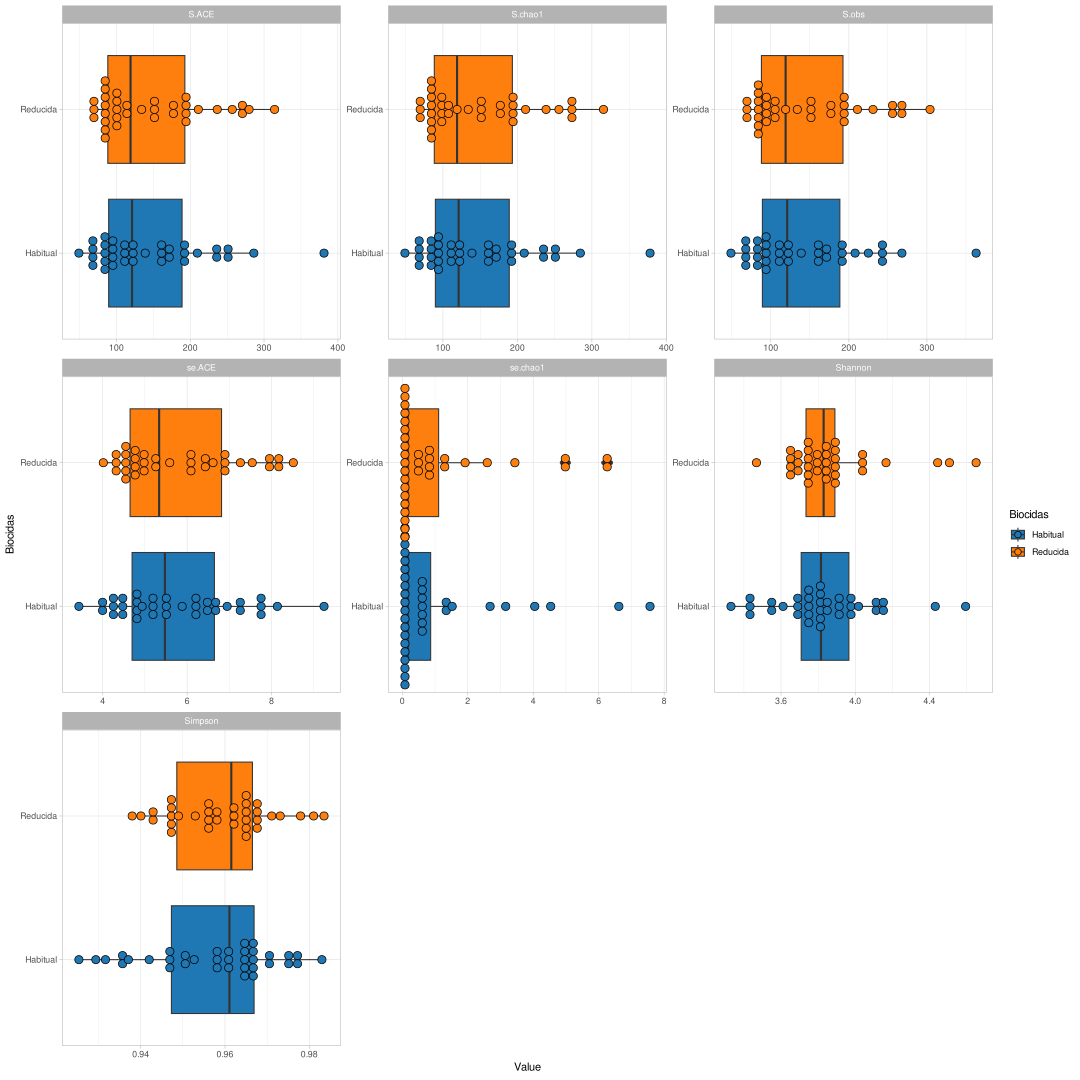
\includegraphics{InformeNeiker_files/figure-pdf/unnamed-chunk-7-2.pdf}

}

\end{figure}

\begin{Shaded}
\begin{Highlighting}[]
\NormalTok{Div }\SpecialCharTok{\%\textgreater{}\%} 
  \FunctionTok{pivot\_longer}\NormalTok{(}\AttributeTok{names\_to =} \StringTok{"Index"}\NormalTok{, }\AttributeTok{values\_to =} \StringTok{"Value"}\NormalTok{, }\SpecialCharTok{{-}}\NormalTok{Sample) }\SpecialCharTok{\%\textgreater{}\%} 
  \FunctionTok{inner\_join}\NormalTok{(metadata }\SpecialCharTok{\%\textgreater{}\%} 
               \FunctionTok{mutate}\NormalTok{(}\AttributeTok{Sample =} \FunctionTok{str\_c}\NormalTok{(}\StringTok{"Sample\_"}\NormalTok{,Sample)) }\SpecialCharTok{\%\textgreater{}\%} 
               \FunctionTok{mutate}\NormalTok{(}\AttributeTok{Combinada =} \FunctionTok{str\_c}\NormalTok{(}\StringTok{\textasciigrave{}}\AttributeTok{Cambio climático}\StringTok{\textasciigrave{}}\NormalTok{,}\StringTok{"+"}\NormalTok{,Biocidas))}
\NormalTok{             ) }\SpecialCharTok{\%\textgreater{}\%} 
  \FunctionTok{filter}\NormalTok{(}\StringTok{\textasciigrave{}}\AttributeTok{Cambio climático}\StringTok{\textasciigrave{}} \SpecialCharTok{==} \StringTok{"Control"} \SpecialCharTok{|} \StringTok{\textasciigrave{}}\AttributeTok{Cambio climático}\StringTok{\textasciigrave{}} \SpecialCharTok{==} \StringTok{"Temperatura elevada"}\NormalTok{) }\SpecialCharTok{\%\textgreater{}\%} 
  \FunctionTok{ggplot}\NormalTok{(}\FunctionTok{aes}\NormalTok{(}\AttributeTok{x =}\NormalTok{ Combinada, }\AttributeTok{y =}\NormalTok{ Value, }\AttributeTok{fill =}\NormalTok{ Combinada)) }\SpecialCharTok{+} 
  \FunctionTok{geom\_boxplot}\NormalTok{() }\SpecialCharTok{+} 
  \FunctionTok{geom\_dotplot}\NormalTok{(}\AttributeTok{binaxis =} \StringTok{"y"}\NormalTok{, }\AttributeTok{stackdir =} \StringTok{"center"}\NormalTok{,}\AttributeTok{shape =} \DecValTok{21}\NormalTok{) }\SpecialCharTok{+}
  \FunctionTok{facet\_wrap}\NormalTok{(}\SpecialCharTok{\textasciitilde{}}\NormalTok{Index, }\AttributeTok{scales =} \StringTok{"free"}\NormalTok{) }\SpecialCharTok{+}
  \FunctionTok{scale\_fill\_d3}\NormalTok{() }\SpecialCharTok{+} 
  \FunctionTok{theme\_light}\NormalTok{() }\SpecialCharTok{+} \FunctionTok{coord\_flip}\NormalTok{()}
\end{Highlighting}
\end{Shaded}

\begin{verbatim}
Joining with `by = join_by(Sample)`
\end{verbatim}

\begin{verbatim}
Warning in geom_dotplot(binaxis = "y", stackdir = "center", shape = 21):
Ignoring unknown parameters: `shape`
\end{verbatim}

\begin{verbatim}
Bin width defaults to 1/30 of the range of the data. Pick better value with
`binwidth`.
\end{verbatim}

\begin{figure}[H]

{\centering 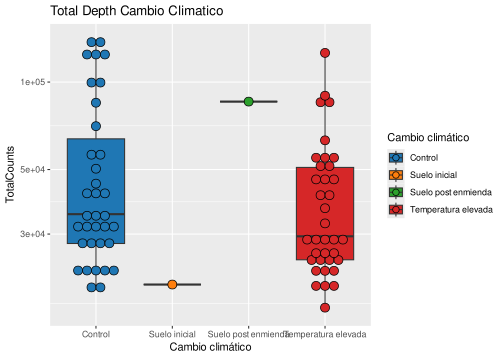
\includegraphics{InformeNeiker_files/figure-pdf/unnamed-chunk-7-3.pdf}

}

\end{figure}

\begin{Shaded}
\begin{Highlighting}[]
\NormalTok{Div }\SpecialCharTok{\%\textgreater{}\%} 
  \FunctionTok{pivot\_longer}\NormalTok{(}\AttributeTok{names\_to =} \StringTok{"Index"}\NormalTok{, }\AttributeTok{values\_to =} \StringTok{"Value"}\NormalTok{, }\SpecialCharTok{{-}}\NormalTok{Sample) }\SpecialCharTok{\%\textgreater{}\%} 
  \FunctionTok{inner\_join}\NormalTok{(metadata }\SpecialCharTok{\%\textgreater{}\%} 
               \FunctionTok{mutate}\NormalTok{(}\AttributeTok{Sample =} \FunctionTok{str\_c}\NormalTok{(}\StringTok{"Sample\_"}\NormalTok{,Sample)) }\SpecialCharTok{\%\textgreater{}\%} 
               \FunctionTok{mutate}\NormalTok{(}\AttributeTok{Combinada =} \FunctionTok{str\_c}\NormalTok{(}\StringTok{\textasciigrave{}}\AttributeTok{Cambio climático}\StringTok{\textasciigrave{}}\NormalTok{,}\StringTok{"+"}\NormalTok{,Biocidas))}
\NormalTok{             ) }\SpecialCharTok{\%\textgreater{}\%} 
  \FunctionTok{filter}\NormalTok{(}\StringTok{\textasciigrave{}}\AttributeTok{Cambio climático}\StringTok{\textasciigrave{}} \SpecialCharTok{==} \StringTok{"Control"} \SpecialCharTok{|} \StringTok{\textasciigrave{}}\AttributeTok{Cambio climático}\StringTok{\textasciigrave{}} \SpecialCharTok{==} \StringTok{"Temperatura elevada"}\NormalTok{) }\SpecialCharTok{\%\textgreater{}\%} 
  \FunctionTok{ggplot}\NormalTok{(}\FunctionTok{aes}\NormalTok{(}\AttributeTok{x =}\NormalTok{ toma, }\AttributeTok{y =}\NormalTok{ Value, }\AttributeTok{fill =}\NormalTok{ toma)) }\SpecialCharTok{+} 
  \FunctionTok{geom\_boxplot}\NormalTok{() }\SpecialCharTok{+} 
  \FunctionTok{geom\_dotplot}\NormalTok{(}\AttributeTok{binaxis =} \StringTok{"y"}\NormalTok{, }\AttributeTok{stackdir =} \StringTok{"center"}\NormalTok{,}\AttributeTok{shape =} \DecValTok{21}\NormalTok{) }\SpecialCharTok{+}
  \FunctionTok{facet\_wrap}\NormalTok{(}\SpecialCharTok{\textasciitilde{}}\NormalTok{Index, }\AttributeTok{scales =} \StringTok{"free"}\NormalTok{) }\SpecialCharTok{+}
  \FunctionTok{scale\_fill\_d3}\NormalTok{() }\SpecialCharTok{+} 
  \FunctionTok{theme\_light}\NormalTok{() }\SpecialCharTok{+} 
  \FunctionTok{theme}\NormalTok{(}\AttributeTok{axis.text =} \FunctionTok{element\_text}\NormalTok{(}\AttributeTok{angle =} \DecValTok{45}\NormalTok{, }\AttributeTok{hjust =} \DecValTok{1}\NormalTok{))}
\end{Highlighting}
\end{Shaded}

\begin{verbatim}
Joining with `by = join_by(Sample)`
\end{verbatim}

\begin{verbatim}
Warning in geom_dotplot(binaxis = "y", stackdir = "center", shape = 21):
Ignoring unknown parameters: `shape`
\end{verbatim}

\begin{verbatim}
Bin width defaults to 1/30 of the range of the data. Pick better value with
`binwidth`.
\end{verbatim}

\begin{figure}[H]

{\centering 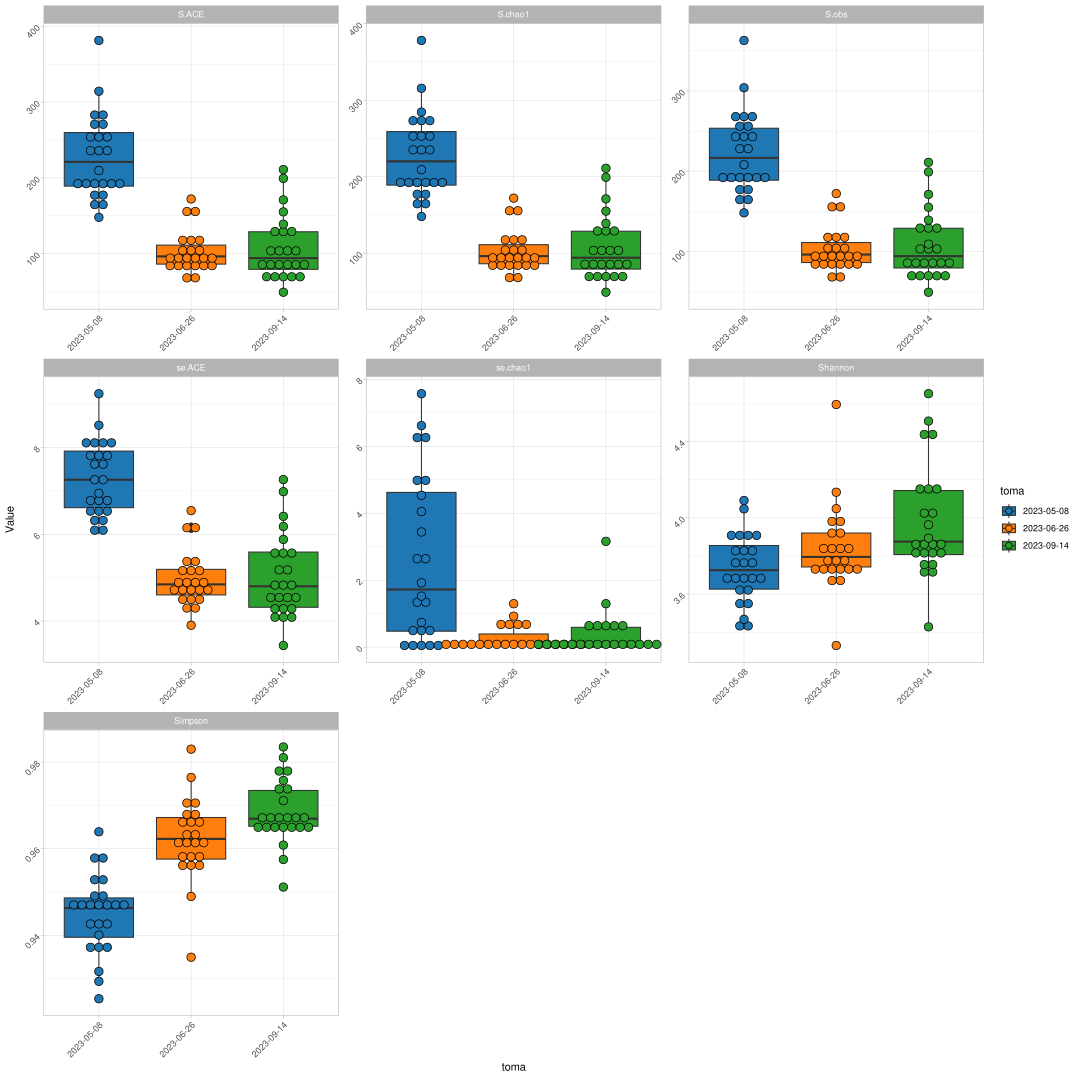
\includegraphics{InformeNeiker_files/figure-pdf/unnamed-chunk-7-4.pdf}

}

\end{figure}

\begin{Shaded}
\begin{Highlighting}[]
\NormalTok{Div }\SpecialCharTok{\%\textgreater{}\%} 
  \FunctionTok{pivot\_longer}\NormalTok{(}\AttributeTok{names\_to =} \StringTok{"Index"}\NormalTok{, }\AttributeTok{values\_to =} \StringTok{"Value"}\NormalTok{, }\SpecialCharTok{{-}}\NormalTok{Sample) }\SpecialCharTok{\%\textgreater{}\%} 
  \FunctionTok{inner\_join}\NormalTok{(metadata }\SpecialCharTok{\%\textgreater{}\%} 
               \FunctionTok{mutate}\NormalTok{(}\AttributeTok{Sample =} \FunctionTok{str\_c}\NormalTok{(}\StringTok{"Sample\_"}\NormalTok{,Sample)) }\SpecialCharTok{\%\textgreater{}\%} 
               \FunctionTok{mutate}\NormalTok{(}\AttributeTok{Combinada =} \FunctionTok{str\_c}\NormalTok{(}\StringTok{\textasciigrave{}}\AttributeTok{Cambio climático}\StringTok{\textasciigrave{}}\NormalTok{,}\StringTok{"+"}\NormalTok{,Biocidas))}
\NormalTok{             ) }\SpecialCharTok{\%\textgreater{}\%} 
  \FunctionTok{filter}\NormalTok{(}\StringTok{\textasciigrave{}}\AttributeTok{Cambio climático}\StringTok{\textasciigrave{}} \SpecialCharTok{==} \StringTok{"Control"} \SpecialCharTok{|} \StringTok{\textasciigrave{}}\AttributeTok{Cambio climático}\StringTok{\textasciigrave{}} \SpecialCharTok{==} \StringTok{"Temperatura elevada"}\NormalTok{) }\SpecialCharTok{\%\textgreater{}\%} 
  \FunctionTok{ggplot}\NormalTok{(}\FunctionTok{aes}\NormalTok{(}\AttributeTok{x =}\NormalTok{ Combinada, }\AttributeTok{y =}\NormalTok{ Value, }\AttributeTok{fill =}\NormalTok{ Combinada)) }\SpecialCharTok{+} 
  \FunctionTok{geom\_boxplot}\NormalTok{() }\SpecialCharTok{+} 
  \FunctionTok{geom\_dotplot}\NormalTok{(}\AttributeTok{binaxis =} \StringTok{"y"}\NormalTok{, }\AttributeTok{stackdir =} \StringTok{"center"}\NormalTok{,}\AttributeTok{shape =} \DecValTok{21}\NormalTok{) }\SpecialCharTok{+}
  \FunctionTok{facet\_wrap}\NormalTok{(toma}\SpecialCharTok{\textasciitilde{}}\NormalTok{Index, }\AttributeTok{scales =} \StringTok{"free"}\NormalTok{) }\SpecialCharTok{+}
  \FunctionTok{scale\_fill\_d3}\NormalTok{() }\SpecialCharTok{+} 
  \FunctionTok{theme\_light}\NormalTok{() }\SpecialCharTok{+} \FunctionTok{coord\_flip}\NormalTok{()}
\end{Highlighting}
\end{Shaded}

\begin{verbatim}
Joining with `by = join_by(Sample)`
\end{verbatim}

\begin{verbatim}
Warning in geom_dotplot(binaxis = "y", stackdir = "center", shape = 21):
Ignoring unknown parameters: `shape`
\end{verbatim}

\begin{verbatim}
Bin width defaults to 1/30 of the range of the data. Pick better value with
`binwidth`.
\end{verbatim}

\begin{figure}[H]

{\centering 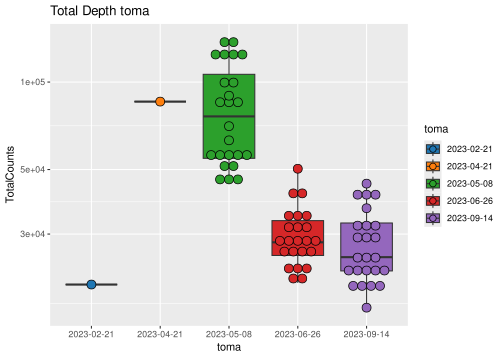
\includegraphics{InformeNeiker_files/figure-pdf/unnamed-chunk-7-5.pdf}

}

\end{figure}

\begin{Shaded}
\begin{Highlighting}[]
\FunctionTok{ggbetweenstats}\NormalTok{(}\AttributeTok{x =}\NormalTok{ Combinada,}
               \AttributeTok{y =}\NormalTok{ S.chao1, }
               \AttributeTok{data =}\NormalTok{ Div }\SpecialCharTok{\%\textgreater{}\%} \FunctionTok{inner\_join}\NormalTok{(metadata }\SpecialCharTok{\%\textgreater{}\%}                                                                       \FunctionTok{filter}\NormalTok{(Sample }\SpecialCharTok{\textless{}} \DecValTok{73}\NormalTok{) }\SpecialCharTok{\%\textgreater{}\%} 
                                \FunctionTok{mutate}\NormalTok{(}\AttributeTok{Sample =} \FunctionTok{str\_c}\NormalTok{(}\StringTok{"Sample\_"}\NormalTok{,Sample)) }\SpecialCharTok{\%\textgreater{}\%} 
                                \FunctionTok{mutate}\NormalTok{(}\AttributeTok{Combinada =} \FunctionTok{str\_c}\NormalTok{(}\StringTok{\textasciigrave{}}\AttributeTok{Cambio climático}\StringTok{\textasciigrave{}}\NormalTok{,}\StringTok{"+"}\NormalTok{,Biocidas))),}
               \AttributeTok{type =} \StringTok{"robust"}\NormalTok{, }\AttributeTok{title =} \StringTok{"Chao Alpha Diversity"}\NormalTok{)}
\end{Highlighting}
\end{Shaded}

\begin{verbatim}
Joining with `by = join_by(Sample)`
\end{verbatim}

\begin{figure}[H]

{\centering 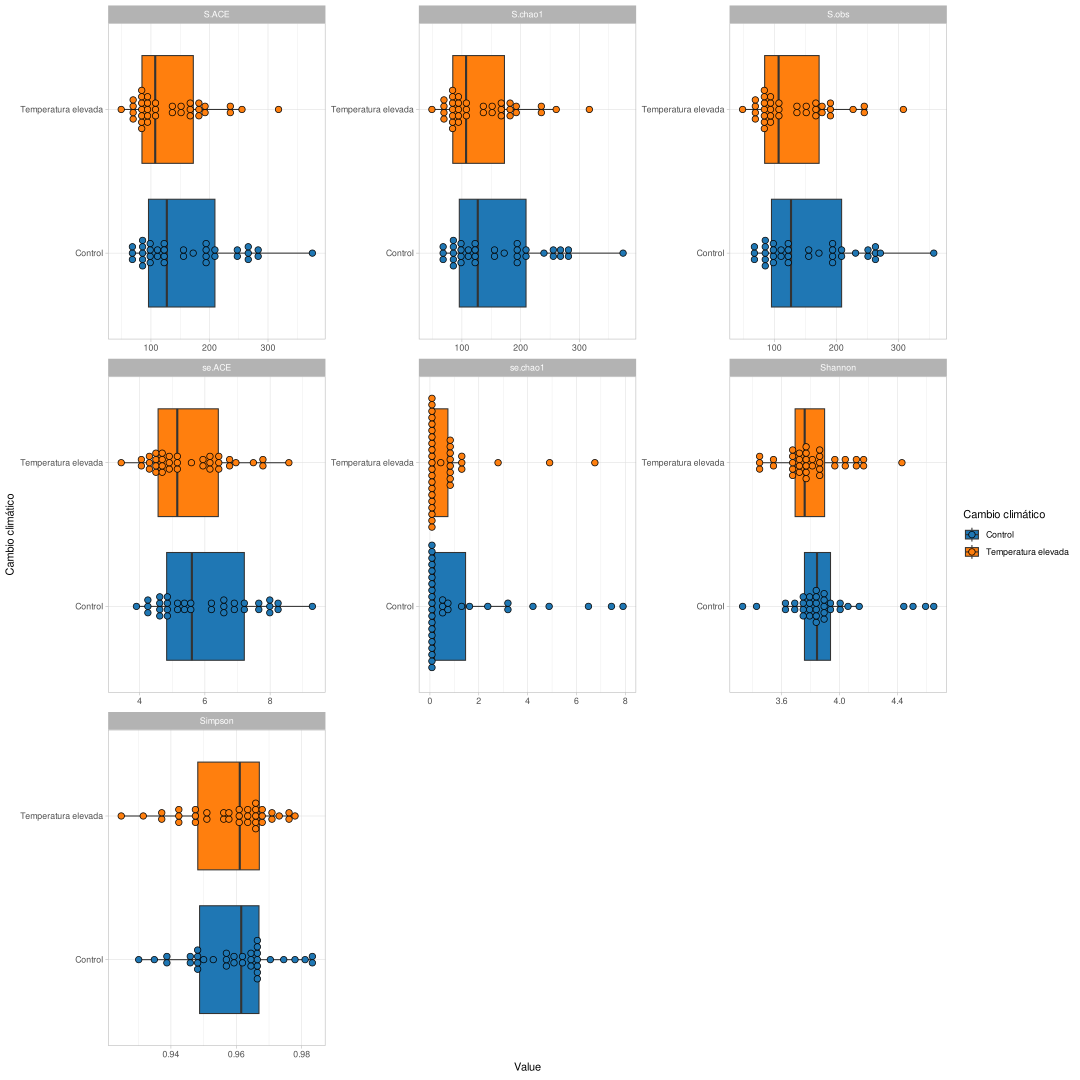
\includegraphics{InformeNeiker_files/figure-pdf/unnamed-chunk-8-1.pdf}

}

\end{figure}

\begin{Shaded}
\begin{Highlighting}[]
\FunctionTok{ggbetweenstats}\NormalTok{(}\AttributeTok{x =}\NormalTok{ toma,}
               \AttributeTok{y =}\NormalTok{ S.chao1, }
               \AttributeTok{data =}\NormalTok{ Div }\SpecialCharTok{\%\textgreater{}\%} \FunctionTok{inner\_join}\NormalTok{(metadata }\SpecialCharTok{\%\textgreater{}\%}                                                                       \FunctionTok{filter}\NormalTok{(Sample }\SpecialCharTok{\textless{}} \DecValTok{73}\NormalTok{) }\SpecialCharTok{\%\textgreater{}\%} 
                                \FunctionTok{mutate}\NormalTok{(}\AttributeTok{Sample =} \FunctionTok{str\_c}\NormalTok{(}\StringTok{"Sample\_"}\NormalTok{,Sample)) }\SpecialCharTok{\%\textgreater{}\%} 
                                \FunctionTok{mutate}\NormalTok{(}\AttributeTok{Combinada =} \FunctionTok{str\_c}\NormalTok{(}\StringTok{\textasciigrave{}}\AttributeTok{Cambio climático}\StringTok{\textasciigrave{}}\NormalTok{,}\StringTok{"+"}\NormalTok{,Biocidas))),}
               \AttributeTok{type =} \StringTok{"robust"}\NormalTok{, }\AttributeTok{title =} \StringTok{"Chao Alpha Diversity"}\NormalTok{)}
\end{Highlighting}
\end{Shaded}

\begin{verbatim}
Joining with `by = join_by(Sample)`
\end{verbatim}

\begin{figure}[H]

{\centering 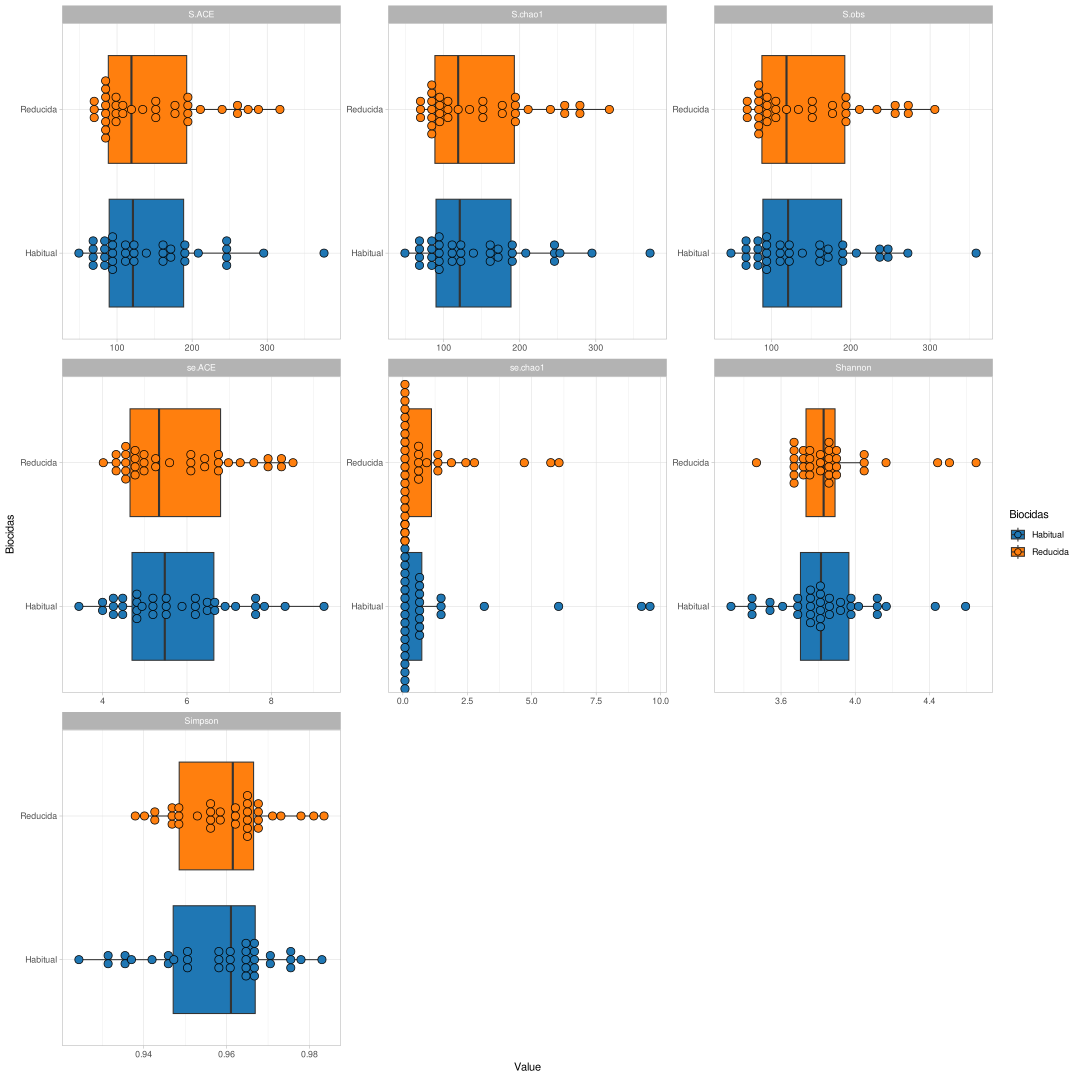
\includegraphics{InformeNeiker_files/figure-pdf/unnamed-chunk-8-2.pdf}

}

\end{figure}

\hypertarget{beta-diversity}{%
\section{Beta Diversity}\label{beta-diversity}}

\begin{Shaded}
\begin{Highlighting}[]
\NormalTok{otu\_table\_sorted }\OtherTok{\textless{}{-}}\NormalTok{ rare\_table }\SpecialCharTok{\%\textgreater{}\%} 
  \FunctionTok{as.data.frame}\NormalTok{() }\SpecialCharTok{\%\textgreater{}\%} 
  \FunctionTok{rownames\_to\_column}\NormalTok{(}\StringTok{"Sample"}\NormalTok{) }\SpecialCharTok{\%\textgreater{}\%} 
  \FunctionTok{inner\_join}\NormalTok{(metadata }\SpecialCharTok{\%\textgreater{}\%} 
               \FunctionTok{filter}\NormalTok{(Sample }\SpecialCharTok{\textless{}} \DecValTok{73}\NormalTok{) }\SpecialCharTok{\%\textgreater{}\%} 
               \FunctionTok{mutate}\NormalTok{(}\AttributeTok{Sample =} \FunctionTok{str\_c}\NormalTok{(}\StringTok{"Sample\_"}\NormalTok{,Sample))) }\SpecialCharTok{\%\textgreater{}\%} 
\NormalTok{  dplyr}\SpecialCharTok{::}\FunctionTok{select}\NormalTok{(}\SpecialCharTok{{-}}\NormalTok{(Subparcela}\SpecialCharTok{:}\NormalTok{toma)) }\SpecialCharTok{\%\textgreater{}\%} \FunctionTok{column\_to\_rownames}\NormalTok{(}\StringTok{"Sample"}\NormalTok{) }\SpecialCharTok{\%\textgreater{}\%} \FunctionTok{as.matrix}\NormalTok{()}
\end{Highlighting}
\end{Shaded}

\begin{verbatim}
Joining with `by = join_by(Sample)`
\end{verbatim}

\begin{Shaded}
\begin{Highlighting}[]
\NormalTok{metadata\_sorted }\OtherTok{\textless{}{-}}\NormalTok{ rare\_table }\SpecialCharTok{\%\textgreater{}\%} 
  \FunctionTok{as.data.frame}\NormalTok{() }\SpecialCharTok{\%\textgreater{}\%} 
  \FunctionTok{rownames\_to\_column}\NormalTok{(}\StringTok{"Sample"}\NormalTok{) }\SpecialCharTok{\%\textgreater{}\%} 
  \FunctionTok{inner\_join}\NormalTok{(metadata }\SpecialCharTok{\%\textgreater{}\%} 
               \FunctionTok{filter}\NormalTok{(Sample }\SpecialCharTok{\textless{}} \DecValTok{73}\NormalTok{) }\SpecialCharTok{\%\textgreater{}\%} 
               \FunctionTok{mutate}\NormalTok{(}\AttributeTok{Sample =} \FunctionTok{str\_c}\NormalTok{(}\StringTok{"Sample\_"}\NormalTok{,Sample)) }\SpecialCharTok{\%\textgreater{}\%} 
               \FunctionTok{mutate}\NormalTok{(}\AttributeTok{Combinada =} \FunctionTok{str\_c}\NormalTok{(}\StringTok{\textasciigrave{}}\AttributeTok{Cambio climático}\StringTok{\textasciigrave{}}\NormalTok{,}\StringTok{"+"}\NormalTok{,Biocidas))) }\SpecialCharTok{\%\textgreater{}\%} 
\NormalTok{  dplyr}\SpecialCharTok{::}\FunctionTok{select}\NormalTok{(Sample,Subparcela}\SpecialCharTok{:}\NormalTok{Combinada,toma) }\SpecialCharTok{\%\textgreater{}\%} \FunctionTok{column\_to\_rownames}\NormalTok{(}\StringTok{"Sample"}\NormalTok{)}
\end{Highlighting}
\end{Shaded}

\begin{verbatim}
Joining with `by = join_by(Sample)`
\end{verbatim}

\begin{Shaded}
\begin{Highlighting}[]
\NormalTok{map }\OtherTok{\textless{}{-}} \FunctionTok{metaMDS}\NormalTok{(otu\_table\_sorted)}
\end{Highlighting}
\end{Shaded}

\begin{verbatim}
Square root transformation
Wisconsin double standardization
Run 0 stress 0.1261215 
Run 1 stress 0.1293506 
Run 2 stress 0.1608379 
Run 3 stress 0.1733755 
Run 4 stress 0.164309 
Run 5 stress 0.1475155 
Run 6 stress 0.167158 
Run 7 stress 0.1572058 
Run 8 stress 0.1664461 
Run 9 stress 0.1565889 
Run 10 stress 0.151448 
Run 11 stress 0.1574007 
Run 12 stress 0.1701131 
Run 13 stress 0.1568002 
Run 14 stress 0.1431316 
Run 15 stress 0.16137 
Run 16 stress 0.1674387 
Run 17 stress 0.1530764 
Run 18 stress 0.1666148 
Run 19 stress 0.1662134 
Run 20 stress 0.155009 
*** Best solution was not repeated -- monoMDS stopping criteria:
    13: stress ratio > sratmax
     7: scale factor of the gradient < sfgrmin
\end{verbatim}

\begin{Shaded}
\begin{Highlighting}[]
\NormalTok{map}\SpecialCharTok{$}\NormalTok{points }\SpecialCharTok{\%\textgreater{}\%} 
  \FunctionTok{as.data.frame}\NormalTok{() }\SpecialCharTok{\%\textgreater{}\%} 
  \FunctionTok{rownames\_to\_column}\NormalTok{(}\StringTok{"Sample"}\NormalTok{) }\SpecialCharTok{\%\textgreater{}\%} 
  \FunctionTok{inner\_join}\NormalTok{(metadata }\SpecialCharTok{\%\textgreater{}\%} 
               \FunctionTok{mutate}\NormalTok{(}\AttributeTok{Sample =} \FunctionTok{str\_c}\NormalTok{(}\StringTok{"Sample\_"}\NormalTok{,Sample)) }\SpecialCharTok{\%\textgreater{}\%} 
               \FunctionTok{mutate}\NormalTok{(}\AttributeTok{Combinada =} \FunctionTok{str\_c}\NormalTok{(}\StringTok{\textasciigrave{}}\AttributeTok{Cambio climático}\StringTok{\textasciigrave{}}\NormalTok{,}\StringTok{"+"}\NormalTok{,Biocidas))) }\SpecialCharTok{\%\textgreater{}\%} 
  \FunctionTok{ggplot}\NormalTok{(}\FunctionTok{aes}\NormalTok{(}\AttributeTok{x =}\NormalTok{ MDS1, }\AttributeTok{y =}\NormalTok{ MDS2, }\AttributeTok{fill =} \StringTok{\textasciigrave{}}\AttributeTok{Cambio climático}\StringTok{\textasciigrave{}}\NormalTok{)) }\SpecialCharTok{+} 
  \FunctionTok{geom\_point}\NormalTok{(}\AttributeTok{shape =} \DecValTok{21}\NormalTok{, }\AttributeTok{size =}\DecValTok{3}\NormalTok{) }\SpecialCharTok{+}
  \FunctionTok{theme\_light}\NormalTok{() }\SpecialCharTok{+}
  \FunctionTok{scale\_fill\_d3}\NormalTok{()}
\end{Highlighting}
\end{Shaded}

\begin{verbatim}
Joining with `by = join_by(Sample)`
\end{verbatim}

\begin{figure}[H]

{\centering 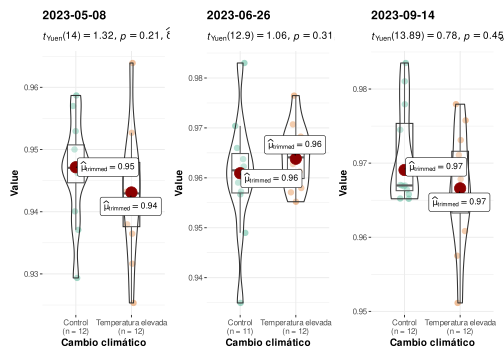
\includegraphics{InformeNeiker_files/figure-pdf/unnamed-chunk-9-1.pdf}

}

\end{figure}

\begin{Shaded}
\begin{Highlighting}[]
\NormalTok{map}\SpecialCharTok{$}\NormalTok{points }\SpecialCharTok{\%\textgreater{}\%} 
  \FunctionTok{as.data.frame}\NormalTok{() }\SpecialCharTok{\%\textgreater{}\%} 
  \FunctionTok{rownames\_to\_column}\NormalTok{(}\StringTok{"Sample"}\NormalTok{) }\SpecialCharTok{\%\textgreater{}\%} 
  \FunctionTok{inner\_join}\NormalTok{(metadata }\SpecialCharTok{\%\textgreater{}\%} 
               \FunctionTok{mutate}\NormalTok{(}\AttributeTok{Sample =} \FunctionTok{str\_c}\NormalTok{(}\StringTok{"Sample\_"}\NormalTok{,Sample)) }\SpecialCharTok{\%\textgreater{}\%} 
               \FunctionTok{mutate}\NormalTok{(}\AttributeTok{Combinada =} \FunctionTok{str\_c}\NormalTok{(}\StringTok{\textasciigrave{}}\AttributeTok{Cambio climático}\StringTok{\textasciigrave{}}\NormalTok{,}\StringTok{"+"}\NormalTok{,Biocidas))) }\SpecialCharTok{\%\textgreater{}\%} 
  \FunctionTok{ggplot}\NormalTok{(}\FunctionTok{aes}\NormalTok{(}\AttributeTok{x =}\NormalTok{ MDS1, }\AttributeTok{y =}\NormalTok{ MDS2, }\AttributeTok{fill =}\NormalTok{ Biocidas)) }\SpecialCharTok{+} 
  \FunctionTok{geom\_point}\NormalTok{(}\AttributeTok{shape =} \DecValTok{21}\NormalTok{, }\AttributeTok{size =}\DecValTok{3}\NormalTok{) }\SpecialCharTok{+}
  \FunctionTok{theme\_light}\NormalTok{() }\SpecialCharTok{+}
  \FunctionTok{scale\_fill\_d3}\NormalTok{()}
\end{Highlighting}
\end{Shaded}

\begin{verbatim}
Joining with `by = join_by(Sample)`
\end{verbatim}

\begin{figure}[H]

{\centering 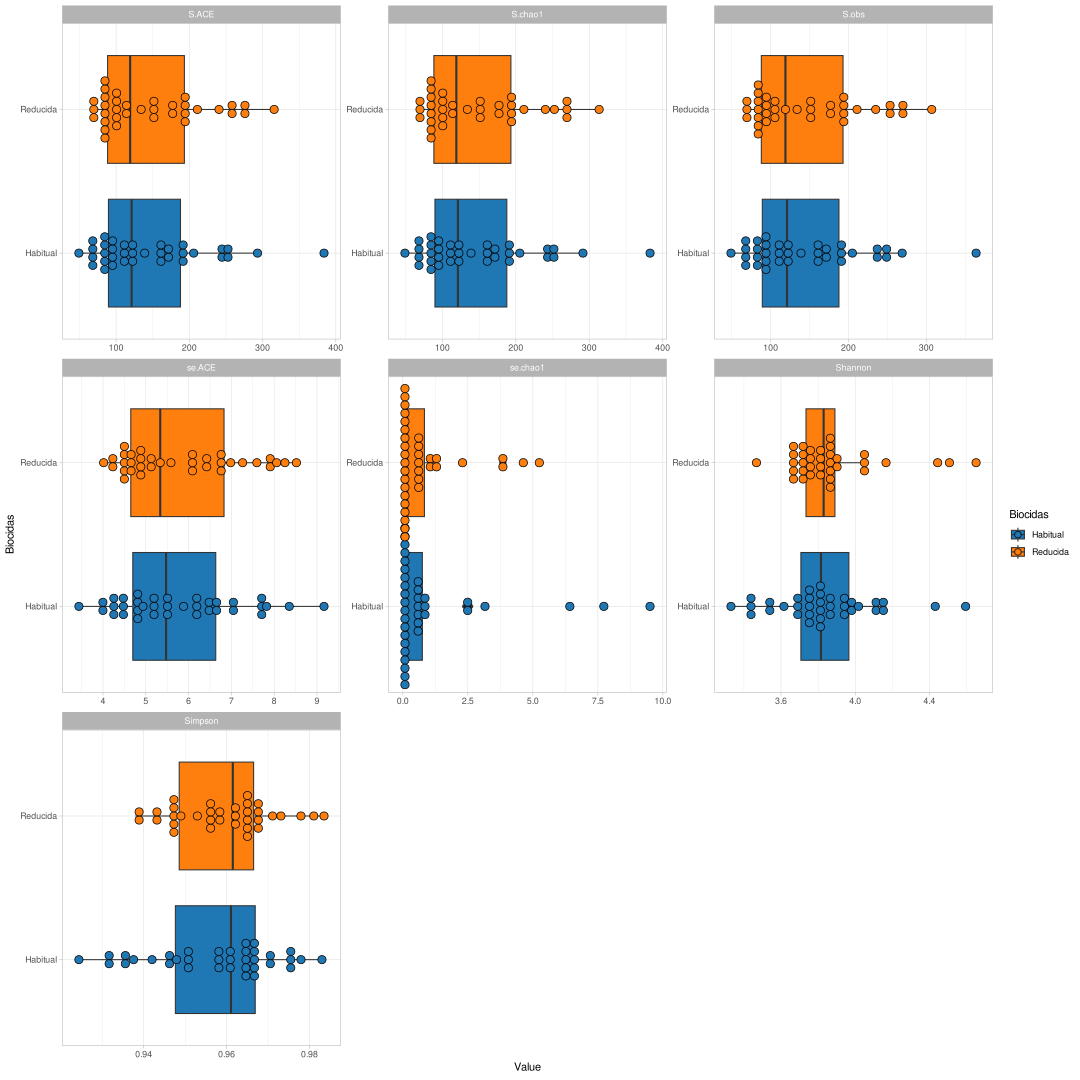
\includegraphics{InformeNeiker_files/figure-pdf/unnamed-chunk-9-2.pdf}

}

\end{figure}

\begin{Shaded}
\begin{Highlighting}[]
\NormalTok{map}\SpecialCharTok{$}\NormalTok{points }\SpecialCharTok{\%\textgreater{}\%} 
  \FunctionTok{as.data.frame}\NormalTok{() }\SpecialCharTok{\%\textgreater{}\%} 
  \FunctionTok{rownames\_to\_column}\NormalTok{(}\StringTok{"Sample"}\NormalTok{) }\SpecialCharTok{\%\textgreater{}\%} 
  \FunctionTok{inner\_join}\NormalTok{(metadata }\SpecialCharTok{\%\textgreater{}\%} 
               \FunctionTok{mutate}\NormalTok{(}\AttributeTok{Sample =} \FunctionTok{str\_c}\NormalTok{(}\StringTok{"Sample\_"}\NormalTok{,Sample)) }\SpecialCharTok{\%\textgreater{}\%} 
               \FunctionTok{mutate}\NormalTok{(}\AttributeTok{Combinada =} \FunctionTok{str\_c}\NormalTok{(}\StringTok{\textasciigrave{}}\AttributeTok{Cambio climático}\StringTok{\textasciigrave{}}\NormalTok{,}\StringTok{"+"}\NormalTok{,Biocidas))) }\SpecialCharTok{\%\textgreater{}\%} 
  \FunctionTok{ggplot}\NormalTok{(}\FunctionTok{aes}\NormalTok{(}\AttributeTok{x =}\NormalTok{ MDS1, }\AttributeTok{y =}\NormalTok{ MDS2, }\AttributeTok{fill =}\NormalTok{ Combinada)) }\SpecialCharTok{+} 
  \FunctionTok{geom\_point}\NormalTok{(}\AttributeTok{shape =} \DecValTok{21}\NormalTok{, }\AttributeTok{size =}\DecValTok{3}\NormalTok{) }\SpecialCharTok{+}
  \FunctionTok{theme\_light}\NormalTok{() }\SpecialCharTok{+}
  \FunctionTok{scale\_fill\_d3}\NormalTok{()}
\end{Highlighting}
\end{Shaded}

\begin{verbatim}
Joining with `by = join_by(Sample)`
\end{verbatim}

\begin{figure}[H]

{\centering 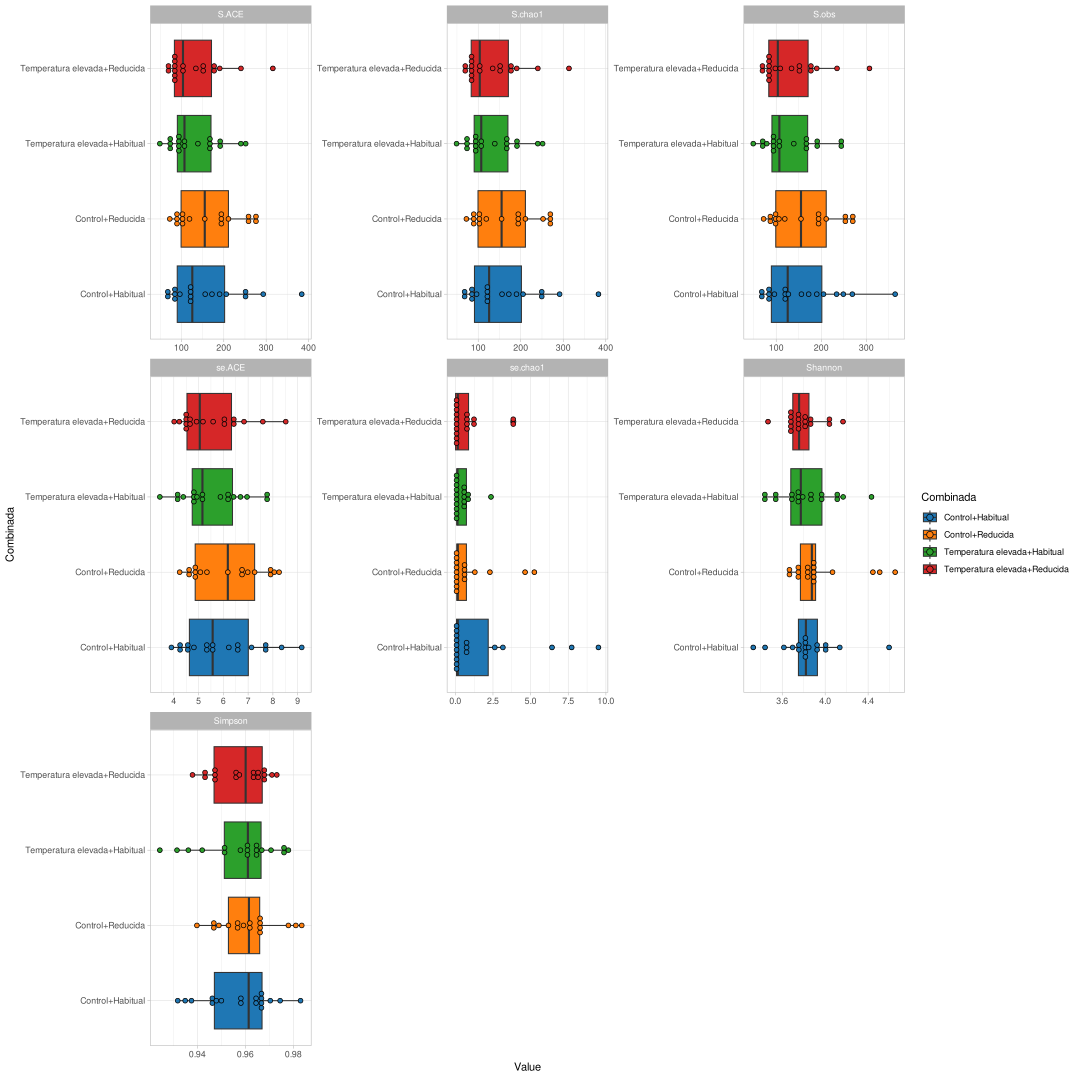
\includegraphics{InformeNeiker_files/figure-pdf/unnamed-chunk-9-3.pdf}

}

\end{figure}

\begin{Shaded}
\begin{Highlighting}[]
\NormalTok{map}\SpecialCharTok{$}\NormalTok{points }\SpecialCharTok{\%\textgreater{}\%} 
  \FunctionTok{as.data.frame}\NormalTok{() }\SpecialCharTok{\%\textgreater{}\%} 
  \FunctionTok{rownames\_to\_column}\NormalTok{(}\StringTok{"Sample"}\NormalTok{) }\SpecialCharTok{\%\textgreater{}\%} 
  \FunctionTok{inner\_join}\NormalTok{(metadata }\SpecialCharTok{\%\textgreater{}\%} 
               \FunctionTok{mutate}\NormalTok{(}\AttributeTok{Sample =} \FunctionTok{str\_c}\NormalTok{(}\StringTok{"Sample\_"}\NormalTok{,Sample)) }\SpecialCharTok{\%\textgreater{}\%} 
               \FunctionTok{mutate}\NormalTok{(}\AttributeTok{Combinada =} \FunctionTok{str\_c}\NormalTok{(}\StringTok{\textasciigrave{}}\AttributeTok{Cambio climático}\StringTok{\textasciigrave{}}\NormalTok{,}\StringTok{"+"}\NormalTok{,Biocidas))) }\SpecialCharTok{\%\textgreater{}\%} 
  \FunctionTok{ggplot}\NormalTok{(}\FunctionTok{aes}\NormalTok{(}\AttributeTok{x =}\NormalTok{ MDS1, }\AttributeTok{y =}\NormalTok{ MDS2, }\AttributeTok{fill =}\NormalTok{ toma)) }\SpecialCharTok{+} 
  \FunctionTok{geom\_point}\NormalTok{(}\AttributeTok{shape =} \DecValTok{21}\NormalTok{, }\AttributeTok{size =}\DecValTok{3}\NormalTok{) }\SpecialCharTok{+}
  \FunctionTok{theme\_light}\NormalTok{() }\SpecialCharTok{+}
  \FunctionTok{scale\_fill\_d3}\NormalTok{()}
\end{Highlighting}
\end{Shaded}

\begin{verbatim}
Joining with `by = join_by(Sample)`
\end{verbatim}

\begin{figure}[H]

{\centering 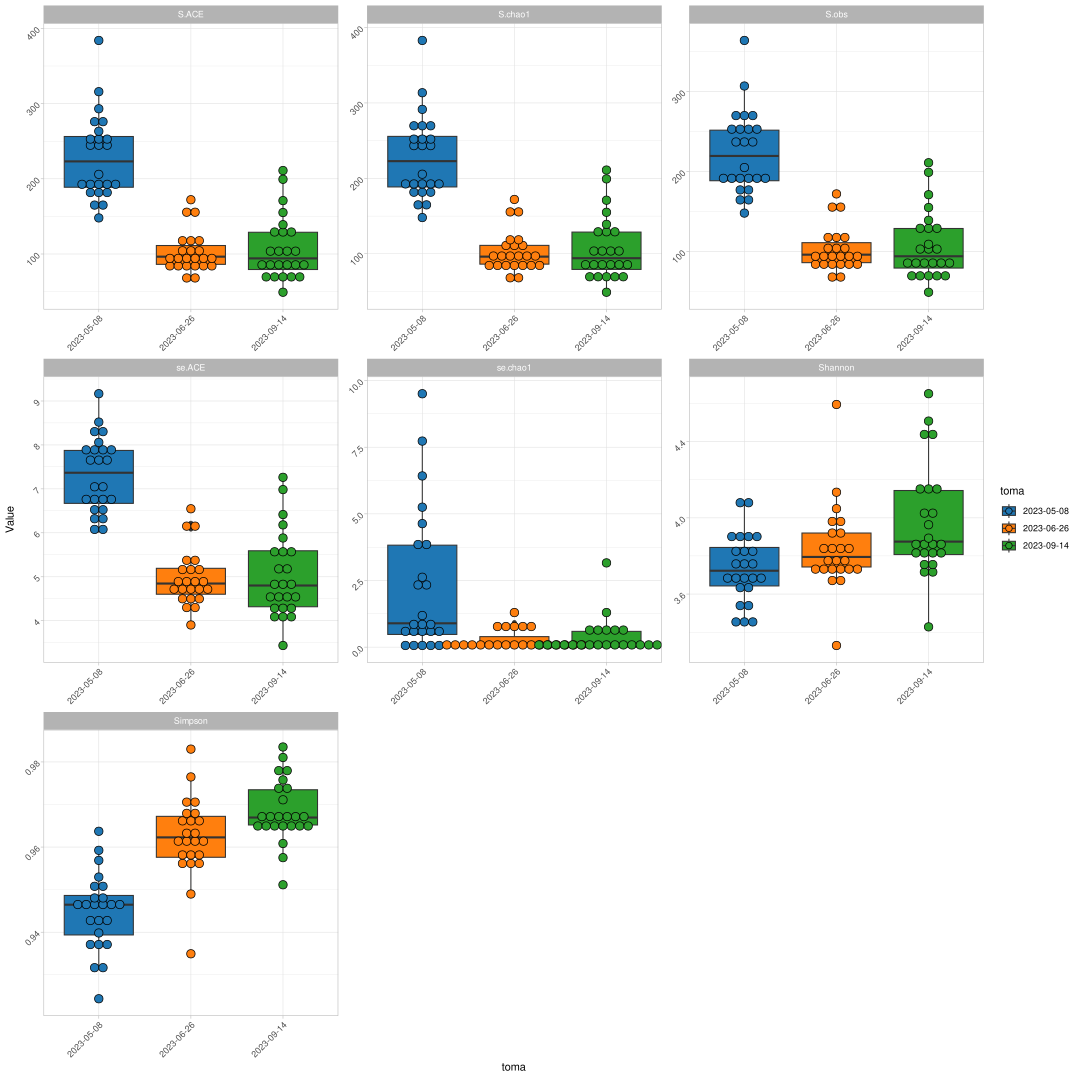
\includegraphics{InformeNeiker_files/figure-pdf/unnamed-chunk-9-4.pdf}

}

\end{figure}

\begin{Shaded}
\begin{Highlighting}[]
\FunctionTok{adonis2}\NormalTok{(otu\_table\_sorted }\SpecialCharTok{\textasciitilde{}}\NormalTok{ Biocidas }\SpecialCharTok{*} \StringTok{\textasciigrave{}}\AttributeTok{Cambio climático}\StringTok{\textasciigrave{}}\NormalTok{, metadata\_sorted,}\AttributeTok{permutations =} \DecValTok{5000}\NormalTok{)}
\end{Highlighting}
\end{Shaded}

\begin{verbatim}
Permutation test for adonis under reduced model
Terms added sequentially (first to last)
Permutation: free
Number of permutations: 5000

adonis2(formula = otu_table_sorted ~ Biocidas * `Cambio climático`, data = metadata_sorted, permutations = 5000)
                            Df SumOfSqs      R2      F Pr(>F)
Biocidas                     1   0.0947 0.00623 0.4313 0.8952
`Cambio climático`           1   0.2796 0.01839 1.2739 0.2174
Biocidas:`Cambio climático`  1   0.1230 0.00809 0.5603 0.7355
Residual                    67  14.7060 0.96729              
Total                       70  15.2033 1.00000              
\end{verbatim}

\begin{Shaded}
\begin{Highlighting}[]
\FunctionTok{adonis2}\NormalTok{(otu\_table\_sorted }\SpecialCharTok{\textasciitilde{}}\NormalTok{ toma }\SpecialCharTok{*}\NormalTok{ Biocidas }\SpecialCharTok{*} \StringTok{\textasciigrave{}}\AttributeTok{Cambio climático}\StringTok{\textasciigrave{}}\NormalTok{, metadata\_sorted, }\AttributeTok{permutations =} \DecValTok{5000}\NormalTok{)}
\end{Highlighting}
\end{Shaded}

\begin{verbatim}
Permutation test for adonis under reduced model
Terms added sequentially (first to last)
Permutation: free
Number of permutations: 5000

adonis2(formula = otu_table_sorted ~ toma * Biocidas * `Cambio climático`, data = metadata_sorted, permutations = 5000)
                                 Df SumOfSqs      R2       F  Pr(>F)    
toma                              2   7.6363 0.50228 35.4114 0.00020 ***
Biocidas                          1   0.0930 0.00612  0.8627 0.41812    
`Cambio climático`                1   0.2745 0.01805  2.5455 0.04619 *  
toma:Biocidas                     2   0.1563 0.01028  0.7250 0.66667    
toma:`Cambio climático`           2   0.3206 0.02109  1.4868 0.14257    
Biocidas:`Cambio climático`       1   0.1229 0.00808  1.1398 0.28574    
toma:Biocidas:`Cambio climático`  2   0.2380 0.01566  1.1038 0.31054    
Residual                         59   6.3616 0.41843                    
Total                            70  15.2033 1.00000                    
---
Signif. codes:  0 '***' 0.001 '**' 0.01 '*' 0.05 '.' 0.1 ' ' 1
\end{verbatim}

\hypertarget{differential-analysis}{%
\section{Differential analysis}\label{differential-analysis}}

\begin{Shaded}
\begin{Highlighting}[]
\NormalTok{test\_table }\OtherTok{\textless{}{-}}\NormalTok{ rare\_table }\SpecialCharTok{\%\textgreater{}\%} 
  \FunctionTok{as.data.frame}\NormalTok{() }\SpecialCharTok{\%\textgreater{}\%} 
  \FunctionTok{rownames\_to\_column}\NormalTok{(}\StringTok{"Sample"}\NormalTok{) }\SpecialCharTok{\%\textgreater{}\%} 
  \FunctionTok{pivot\_longer}\NormalTok{(}\AttributeTok{names\_to =} \StringTok{"Gene"}\NormalTok{, }\AttributeTok{values\_to =} \StringTok{"Abundance"}\NormalTok{, }\SpecialCharTok{{-}}\NormalTok{Sample) }\SpecialCharTok{\%\textgreater{}\%} 
  \FunctionTok{inner\_join}\NormalTok{(metadata }\SpecialCharTok{\%\textgreater{}\%} 
               \FunctionTok{filter}\NormalTok{(Sample }\SpecialCharTok{\textless{}} \DecValTok{73}\NormalTok{) }\SpecialCharTok{\%\textgreater{}\%} 
               \FunctionTok{mutate}\NormalTok{(}\AttributeTok{Sample =} \FunctionTok{str\_c}\NormalTok{(}\StringTok{"Sample\_"}\NormalTok{,Sample)) }\SpecialCharTok{\%\textgreater{}\%} 
               \FunctionTok{mutate}\NormalTok{(}\AttributeTok{Combinada =} \FunctionTok{str\_c}\NormalTok{(}\StringTok{\textasciigrave{}}\AttributeTok{Cambio climático}\StringTok{\textasciigrave{}}\NormalTok{,}\StringTok{"+"}\NormalTok{,Biocidas))) }\SpecialCharTok{\%\textgreater{}\%} 
\NormalTok{  dplyr}\SpecialCharTok{::}\FunctionTok{select}\NormalTok{(}\SpecialCharTok{{-}}\NormalTok{Otros) }\SpecialCharTok{\%\textgreater{}\%} 
  \FunctionTok{group\_by}\NormalTok{(Sample) }\SpecialCharTok{\%\textgreater{}\%} 
  \FunctionTok{mutate}\NormalTok{(}\AttributeTok{TotalAbundance =} \FunctionTok{sum}\NormalTok{(Abundance)) }\SpecialCharTok{\%\textgreater{}\%} 
  \FunctionTok{ungroup}\NormalTok{() }\SpecialCharTok{\%\textgreater{}\%} 
  \FunctionTok{mutate}\NormalTok{(}\AttributeTok{Freq =}\NormalTok{ (Abundance }\SpecialCharTok{+}\DecValTok{1}\NormalTok{) }\SpecialCharTok{/}\NormalTok{TotalAbundance) }\SpecialCharTok{\%\textgreater{}\%} 
  \FunctionTok{mutate}\NormalTok{(}\AttributeTok{Ab2 =}\NormalTok{ Abundance }\SpecialCharTok{+}\DecValTok{1}\NormalTok{) }\SpecialCharTok{\%\textgreater{}\%} 
  \FunctionTok{group\_by}\NormalTok{(Gene) }\SpecialCharTok{\%\textgreater{}\%} 
  \FunctionTok{mutate}\NormalTok{(}\AttributeTok{NZeros =} \FunctionTok{sum}\NormalTok{(Abundance }\SpecialCharTok{==}\DecValTok{0}\NormalTok{)) }\SpecialCharTok{\%\textgreater{}\%} 
  \FunctionTok{filter}\NormalTok{(NZeros }\SpecialCharTok{\textless{}} \DecValTok{10}\NormalTok{) }\SpecialCharTok{\%\textgreater{}\%} 
  \FunctionTok{ungroup}\NormalTok{() }\SpecialCharTok{\%\textgreater{}\%} 
  \FunctionTok{nest\_by}\NormalTok{(Gene) }\SpecialCharTok{\%\textgreater{}\%} 
  \FunctionTok{mutate}\NormalTok{(}\AttributeTok{model\_full =} \FunctionTok{list}\NormalTok{(}\FunctionTok{gamlss}\NormalTok{(Freq }\SpecialCharTok{\textasciitilde{}}\NormalTok{ toma }\SpecialCharTok{+} \StringTok{\textasciigrave{}}\AttributeTok{Cambio climático}\StringTok{\textasciigrave{}} \SpecialCharTok{+}\NormalTok{ Biocidas, }
                             \AttributeTok{data =}\NormalTok{ data,}
                             \AttributeTok{family =} \StringTok{"BE"}\NormalTok{, }
                             \AttributeTok{control =} \FunctionTok{gamlss.control}\NormalTok{(}\AttributeTok{n.cyc =} \DecValTok{200}\NormalTok{, }\AttributeTok{trace =}\NormalTok{ F)))) }\SpecialCharTok{\%\textgreater{}\%} 
  \FunctionTok{mutate}\NormalTok{(}\AttributeTok{model\_reduced =} \FunctionTok{list}\NormalTok{(}\FunctionTok{gamlss}\NormalTok{(Freq }\SpecialCharTok{\textasciitilde{}} \DecValTok{1}\NormalTok{, }
                             \AttributeTok{data =}\NormalTok{ data,}
                             \AttributeTok{family =} \StringTok{"BE"}\NormalTok{, }
                             \AttributeTok{control =} \FunctionTok{gamlss.control}\NormalTok{(}\AttributeTok{n.cyc =} \DecValTok{200}\NormalTok{, }\AttributeTok{trace =}\NormalTok{ F)))) }\SpecialCharTok{\%\textgreater{}\%}
  \FunctionTok{mutate}\NormalTok{(}\AttributeTok{LRT =} \FunctionTok{list}\NormalTok{(}\FunctionTok{test\_lrt}\NormalTok{(model\_full,model\_reduced)))}
\end{Highlighting}
\end{Shaded}

\begin{verbatim}
Joining with `by = join_by(Sample)`
\end{verbatim}

\begin{verbatim}
Warning: There were 6 warnings in `mutate()`.
The first warning was:
i In argument: `LRT = list(test_lrt(model_full, model_reduced))`.
i In row 1.
Caused by warning:
! reiniciar evaluación premisa interrumpida
i Run `dplyr::last_dplyr_warnings()` to see the 5 remaining warnings.
\end{verbatim}

\begin{Shaded}
\begin{Highlighting}[]
\NormalTok{test\_table }\SpecialCharTok{\%\textgreater{}\%} 
\NormalTok{  dplyr}\SpecialCharTok{::}\FunctionTok{select}\NormalTok{(Gene,LRT) }\SpecialCharTok{\%\textgreater{}\%} 
  \FunctionTok{unnest}\NormalTok{(LRT) }\SpecialCharTok{\%\textgreater{}\%} 
  \FunctionTok{drop\_na}\NormalTok{() }\SpecialCharTok{\%\textgreater{}\%} 
  \FunctionTok{mutate}\NormalTok{(}\AttributeTok{padj =} \FunctionTok{p.adjust}\NormalTok{(p,}\AttributeTok{method =} \StringTok{"fdr"}\NormalTok{)) }\SpecialCharTok{\%\textgreater{}\%} 
  \FunctionTok{filter}\NormalTok{(padj }\SpecialCharTok{\textless{}} \FloatTok{0.05}\NormalTok{) }\SpecialCharTok{\%\textgreater{}\%} 
  \FunctionTok{inner\_join}\NormalTok{(labels, }\AttributeTok{by=} \FunctionTok{c}\NormalTok{(}\StringTok{"Gene"}\OtherTok{=}\StringTok{"template"}\NormalTok{)) }\SpecialCharTok{\%\textgreater{}\%} 
  \FunctionTok{relocate}\NormalTok{(label)}
\end{Highlighting}
\end{Shaded}

\begin{verbatim}
# A tibble: 28 x 9
# Groups:   Gene [28]
   label Gene     Name          Model     df df_diff  Chi2        p     padj
   <chr> <chr>    <chr>         <chr>  <int>   <int> <dbl>    <dbl>    <dbl>
 1 arsC  CCQ44981 model_reduced gamlss     2      -4  41.9 1.75e- 8 1.75e- 8
 2 arsC  CDG35806 model_reduced gamlss     2      -4  59.9 3.07e-12 3.07e-12
 3 G2alt EEK74285 model_reduced gamlss     2      -4  23.1 1.24e- 4 1.24e- 4
 4 arsB  EEL98871 model_reduced gamlss     2      -4  37.2 1.61e- 7 1.61e- 7
 5 blt   EJR29024 model_reduced gamlss     2      -4  62.9 7.07e-13 7.07e-13
 6 blt   EJS64113 model_reduced gamlss     2      -4  72.1 8.22e-15 8.22e-15
 7 bfrA  EOT00044 model_reduced gamlss     2      -4  69.8 2.53e-14 2.53e-14
 8 bfrA  GHB15244 model_reduced gamlss     2      -4  18.7 8.80e- 4 8.80e- 4
 9 arsC  KQN89251 model_reduced gamlss     2      -4  40.2 3.99e- 8 3.99e- 8
10 acn   KRD20404 model_reduced gamlss     2      -4 102.  2.98e-21 2.98e-21
# i 18 more rows
\end{verbatim}

\begin{Shaded}
\begin{Highlighting}[]
\NormalTok{significativos }\OtherTok{\textless{}{-}}\NormalTok{ test\_table }\SpecialCharTok{\%\textgreater{}\%} 
\NormalTok{  dplyr}\SpecialCharTok{::}\FunctionTok{select}\NormalTok{(Gene,LRT) }\SpecialCharTok{\%\textgreater{}\%} 
  \FunctionTok{unnest}\NormalTok{(LRT) }\SpecialCharTok{\%\textgreater{}\%} 
  \FunctionTok{drop\_na}\NormalTok{() }\SpecialCharTok{\%\textgreater{}\%} 
  \FunctionTok{mutate}\NormalTok{(}\AttributeTok{padj =} \FunctionTok{p.adjust}\NormalTok{(p,}\AttributeTok{method =} \StringTok{"fdr"}\NormalTok{)) }\SpecialCharTok{\%\textgreater{}\%} 
  \FunctionTok{filter}\NormalTok{(padj }\SpecialCharTok{\textless{}} \FloatTok{0.05}\NormalTok{) }\SpecialCharTok{\%\textgreater{}\%} 
  \FunctionTok{select}\NormalTok{(Gene)}
\end{Highlighting}
\end{Shaded}

\begin{Shaded}
\begin{Highlighting}[]
\NormalTok{test\_table }\SpecialCharTok{\%\textgreater{}\%} 
  \FunctionTok{semi\_join}\NormalTok{(significativos) }\SpecialCharTok{\%\textgreater{}\%}  
  \FunctionTok{mutate}\NormalTok{(}\AttributeTok{contrast =} \FunctionTok{list}\NormalTok{(}\FunctionTok{emmeans}\NormalTok{(model\_full, }
                                 \AttributeTok{specs =} \StringTok{"toma"}\NormalTok{, }
                                 \AttributeTok{data =}\NormalTok{ data)}\SpecialCharTok{\%\textgreater{}\%} 
                       \FunctionTok{pairs}\NormalTok{() }\SpecialCharTok{\%\textgreater{}\%} 
                       \FunctionTok{as.data.frame}\NormalTok{())) }\SpecialCharTok{\%\textgreater{}\%} 
\NormalTok{  dplyr}\SpecialCharTok{::}\FunctionTok{select}\NormalTok{(Gene,contrast) }\SpecialCharTok{\%\textgreater{}\%} 
  \FunctionTok{unnest}\NormalTok{(contrast) }\SpecialCharTok{\%\textgreater{}\%} 
  \FunctionTok{ungroup}\NormalTok{() }\SpecialCharTok{\%\textgreater{}\%} 
  \FunctionTok{mutate}\NormalTok{(}\AttributeTok{p.adj =} \FunctionTok{p.adjust}\NormalTok{(p.value, }\AttributeTok{method =} \StringTok{"fdr"}\NormalTok{)) }\SpecialCharTok{\%\textgreater{}\%}
  \FunctionTok{filter}\NormalTok{(p.adj }\SpecialCharTok{\textless{}} \FloatTok{0.05}\NormalTok{) }\SpecialCharTok{\%\textgreater{}\%} 
  \FunctionTok{separate}\NormalTok{(contrast, }\FunctionTok{c}\NormalTok{(}\StringTok{"group1"}\NormalTok{,}\StringTok{"group2"}\NormalTok{)) }
\end{Highlighting}
\end{Shaded}

\begin{verbatim}
Joining with `by = join_by(Gene)`
\end{verbatim}

\begin{verbatim}
Warning: Expected 2 pieces. Additional pieces discarded in 61 rows [1, 2, 3, 4, 5, 6, 7,
8, 9, 10, 11, 12, 13, 14, 15, 16, 17, 18, 19, 20, ...].
\end{verbatim}

\begin{verbatim}
# A tibble: 61 x 9
   Gene     group1 group2 estimate    SE    df z.ratio  p.value    p.adj
   <chr>    <chr>  <chr>     <dbl> <dbl> <dbl>   <dbl>    <dbl>    <dbl>
 1 CCQ44981 ""     2023     -1.36  0.200   Inf   -6.81 2.91e-11 8.73e-11
 2 CCQ44981 ""     2023     -0.870 0.180   Inf   -4.84 3.85e- 6 7.89e- 6
 3 CDG35806 ""     2023     -1.21  0.156   Inf   -7.75 4.55e-14 1.66e-13
 4 CDG35806 ""     2023     -0.951 0.160   Inf   -5.95 7.83e- 9 1.93e- 8
 5 EEK74285 ""     2023     -0.872 0.216   Inf   -4.04 1.61e- 4 2.87e- 4
 6 EEK74285 ""     2023     -0.932 0.213   Inf   -4.38 3.54e- 5 6.76e- 5
 7 EEL98871 ""     2023     -0.770 0.209   Inf   -3.69 6.58e- 4 1.06e- 3
 8 EEL98871 ""     2023     -1.09  0.198   Inf   -5.52 9.92e- 8 2.38e- 7
 9 EJR29024 ""     2023     -1.08  0.147   Inf   -7.36 5.76e-13 1.93e-12
10 EJR29024 ""     2023     -1.07  0.147   Inf   -7.31 8.39e-13 2.71e-12
# i 51 more rows
\end{verbatim}

\begin{Shaded}
\begin{Highlighting}[]
\NormalTok{significativos }\OtherTok{\textless{}{-}}\NormalTok{ test\_table }\SpecialCharTok{\%\textgreater{}\%} 
\NormalTok{  dplyr}\SpecialCharTok{::}\FunctionTok{select}\NormalTok{(Gene,LRT) }\SpecialCharTok{\%\textgreater{}\%} 
  \FunctionTok{unnest}\NormalTok{(LRT) }\SpecialCharTok{\%\textgreater{}\%} 
  \FunctionTok{drop\_na}\NormalTok{() }\SpecialCharTok{\%\textgreater{}\%} 
  \FunctionTok{mutate}\NormalTok{(}\AttributeTok{padj =} \FunctionTok{p.adjust}\NormalTok{(p,}\AttributeTok{method =} \StringTok{"fdr"}\NormalTok{)) }\SpecialCharTok{\%\textgreater{}\%} 
  \FunctionTok{filter}\NormalTok{(padj }\SpecialCharTok{\textless{}} \FloatTok{0.05}\NormalTok{) }\SpecialCharTok{\%\textgreater{}\%} \FunctionTok{pull}\NormalTok{(Gene)}

\NormalTok{test\_table }\SpecialCharTok{\%\textgreater{}\%} 
  \FunctionTok{filter}\NormalTok{(Gene }\SpecialCharTok{\%in\%}\NormalTok{ significativos) }\SpecialCharTok{\%\textgreater{}\%} 
  \FunctionTok{inner\_join}\NormalTok{(full\_tabla }\SpecialCharTok{\%\textgreater{}\%} 
               \FunctionTok{mutate}\NormalTok{(}\AttributeTok{label =} \FunctionTok{ifelse}\NormalTok{(database }\SpecialCharTok{==}\StringTok{"BAC"}\NormalTok{,}\FunctionTok{str\_c}\NormalTok{(Gene\_name,template, }\AttributeTok{sep=}\StringTok{"|"}\NormalTok{),template)) }\SpecialCharTok{\%\textgreater{}\%}\NormalTok{ dplyr}\SpecialCharTok{::}\FunctionTok{select}\NormalTok{(template,label) }\SpecialCharTok{\%\textgreater{}\%} \FunctionTok{distinct}\NormalTok{(), }\AttributeTok{by =} \FunctionTok{c}\NormalTok{(}\StringTok{"Gene"} \OtherTok{=} \StringTok{"template"}\NormalTok{)) }\SpecialCharTok{\%\textgreater{}\%} 
\NormalTok{  dplyr}\SpecialCharTok{::}\FunctionTok{select}\NormalTok{(Gene,data,label) }\SpecialCharTok{\%\textgreater{}\%} 
  \FunctionTok{unnest}\NormalTok{(data) }\SpecialCharTok{\%\textgreater{}\%} 
  \FunctionTok{ggplot}\NormalTok{(}\FunctionTok{aes}\NormalTok{(}\AttributeTok{x=}\NormalTok{ toma, }\AttributeTok{y =}\NormalTok{ Abundance, }\AttributeTok{fill =}\NormalTok{ toma)) }\SpecialCharTok{+} 
  \FunctionTok{geom\_violin}\NormalTok{() }\SpecialCharTok{+}
  \FunctionTok{geom\_dotplot}\NormalTok{(}\AttributeTok{binaxis =} \StringTok{"y"}\NormalTok{, }\AttributeTok{stackdir =} \StringTok{"center"}\NormalTok{,}\AttributeTok{shape =} \DecValTok{21}\NormalTok{) }\SpecialCharTok{+}
  \FunctionTok{facet\_wrap}\NormalTok{(}\SpecialCharTok{\textasciitilde{}}\NormalTok{label, }\AttributeTok{scales =} \StringTok{"free"}\NormalTok{) }\SpecialCharTok{+}
  \FunctionTok{scale\_fill\_d3}\NormalTok{() }\SpecialCharTok{+} 
  \FunctionTok{theme}\NormalTok{(}\AttributeTok{axis.text.x =} \FunctionTok{element\_text}\NormalTok{(}\AttributeTok{angle =} \DecValTok{25}\NormalTok{, }\AttributeTok{hjust =} \DecValTok{1}\NormalTok{))}
\end{Highlighting}
\end{Shaded}

\begin{verbatim}
Warning in geom_dotplot(binaxis = "y", stackdir = "center", shape = 21):
Ignoring unknown parameters: `shape`
\end{verbatim}

\begin{verbatim}
Bin width defaults to 1/30 of the range of the data. Pick better value with
`binwidth`.
\end{verbatim}

\begin{figure}[H]

{\centering 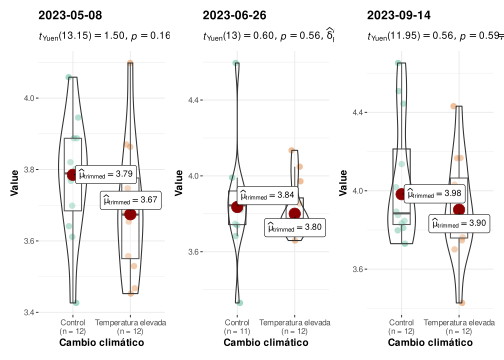
\includegraphics{InformeNeiker_files/figure-pdf/unnamed-chunk-12-1.pdf}

}

\end{figure}

\begin{Shaded}
\begin{Highlighting}[]
\NormalTok{test\_table }\SpecialCharTok{\%\textgreater{}\%} 
  \FunctionTok{filter}\NormalTok{(Gene }\SpecialCharTok{\%in\%}\NormalTok{ significativos) }\SpecialCharTok{\%\textgreater{}\%} 
  \FunctionTok{inner\_join}\NormalTok{(full\_tabla }\SpecialCharTok{\%\textgreater{}\%} 
               \FunctionTok{mutate}\NormalTok{(}\AttributeTok{label =} \FunctionTok{ifelse}\NormalTok{(database }\SpecialCharTok{==}\StringTok{"BAC"}\NormalTok{,}\FunctionTok{str\_c}\NormalTok{(Gene\_name,template, }\AttributeTok{sep=}\StringTok{"|"}\NormalTok{),template)) }\SpecialCharTok{\%\textgreater{}\%}\NormalTok{ dplyr}\SpecialCharTok{::}\FunctionTok{select}\NormalTok{(template,label) }\SpecialCharTok{\%\textgreater{}\%} \FunctionTok{distinct}\NormalTok{(), }\AttributeTok{by =} \FunctionTok{c}\NormalTok{(}\StringTok{"Gene"} \OtherTok{=} \StringTok{"template"}\NormalTok{)) }\SpecialCharTok{\%\textgreater{}\%} 
\NormalTok{  dplyr}\SpecialCharTok{::}\FunctionTok{select}\NormalTok{(Gene,data,label) }\SpecialCharTok{\%\textgreater{}\%} 
  \FunctionTok{unnest}\NormalTok{(data) }\SpecialCharTok{\%\textgreater{}\%} 
  \FunctionTok{ggplot}\NormalTok{(}\FunctionTok{aes}\NormalTok{(}\AttributeTok{x=}\NormalTok{ Biocidas, }\AttributeTok{y =}\NormalTok{ Abundance, }\AttributeTok{fill =}\NormalTok{ Biocidas)) }\SpecialCharTok{+} 
  \FunctionTok{geom\_violin}\NormalTok{() }\SpecialCharTok{+}
  \FunctionTok{geom\_dotplot}\NormalTok{(}\AttributeTok{binaxis =} \StringTok{"y"}\NormalTok{, }\AttributeTok{stackdir =} \StringTok{"center"}\NormalTok{,}\AttributeTok{shape =} \DecValTok{21}\NormalTok{) }\SpecialCharTok{+}
  \FunctionTok{facet\_wrap}\NormalTok{(}\SpecialCharTok{\textasciitilde{}}\NormalTok{label, }\AttributeTok{scales =} \StringTok{"free"}\NormalTok{) }\SpecialCharTok{+}
  \FunctionTok{scale\_fill\_d3}\NormalTok{() }\SpecialCharTok{+} 
  \FunctionTok{theme}\NormalTok{(}\AttributeTok{axis.text.x =} \FunctionTok{element\_text}\NormalTok{(}\AttributeTok{angle =} \DecValTok{25}\NormalTok{, }\AttributeTok{hjust =} \DecValTok{1}\NormalTok{))}
\end{Highlighting}
\end{Shaded}

\begin{verbatim}
Warning in geom_dotplot(binaxis = "y", stackdir = "center", shape = 21):
Ignoring unknown parameters: `shape`
\end{verbatim}

\begin{verbatim}
Bin width defaults to 1/30 of the range of the data. Pick better value with
`binwidth`.
\end{verbatim}

\begin{figure}[H]

{\centering 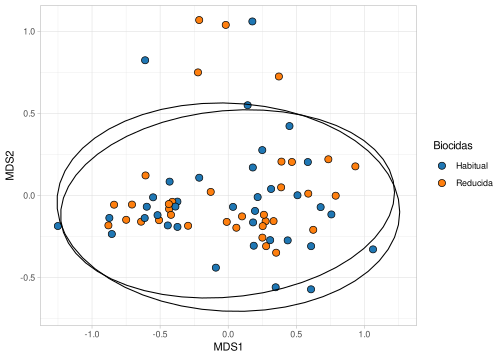
\includegraphics{InformeNeiker_files/figure-pdf/unnamed-chunk-12-2.pdf}

}

\end{figure}

\begin{Shaded}
\begin{Highlighting}[]
\NormalTok{test\_table }\SpecialCharTok{\%\textgreater{}\%} 
  \FunctionTok{filter}\NormalTok{(Gene }\SpecialCharTok{\%in\%}\NormalTok{ significativos) }\SpecialCharTok{\%\textgreater{}\%} 
  \FunctionTok{inner\_join}\NormalTok{(full\_tabla }\SpecialCharTok{\%\textgreater{}\%} 
               \FunctionTok{mutate}\NormalTok{(}\AttributeTok{label =} \FunctionTok{ifelse}\NormalTok{(database }\SpecialCharTok{==}\StringTok{"BAC"}\NormalTok{,}\FunctionTok{str\_c}\NormalTok{(Gene\_name,template, }\AttributeTok{sep=}\StringTok{"|"}\NormalTok{),template)) }\SpecialCharTok{\%\textgreater{}\%}\NormalTok{ dplyr}\SpecialCharTok{::}\FunctionTok{select}\NormalTok{(template,label) }\SpecialCharTok{\%\textgreater{}\%} \FunctionTok{distinct}\NormalTok{(), }\AttributeTok{by =} \FunctionTok{c}\NormalTok{(}\StringTok{"Gene"} \OtherTok{=} \StringTok{"template"}\NormalTok{)) }\SpecialCharTok{\%\textgreater{}\%} 
\NormalTok{  dplyr}\SpecialCharTok{::}\FunctionTok{select}\NormalTok{(Gene,data,label) }\SpecialCharTok{\%\textgreater{}\%} 
  \FunctionTok{unnest}\NormalTok{(data) }\SpecialCharTok{\%\textgreater{}\%} 
  \FunctionTok{ggplot}\NormalTok{(}\FunctionTok{aes}\NormalTok{(}\AttributeTok{x=} \StringTok{\textasciigrave{}}\AttributeTok{Cambio climático}\StringTok{\textasciigrave{}}\NormalTok{, }\AttributeTok{y =}\NormalTok{ Abundance, }\AttributeTok{fill =} \StringTok{\textasciigrave{}}\AttributeTok{Cambio climático}\StringTok{\textasciigrave{}}\NormalTok{)) }\SpecialCharTok{+} 
  \FunctionTok{geom\_violin}\NormalTok{() }\SpecialCharTok{+}
  \FunctionTok{geom\_dotplot}\NormalTok{(}\AttributeTok{binaxis =} \StringTok{"y"}\NormalTok{, }\AttributeTok{stackdir =} \StringTok{"center"}\NormalTok{,}\AttributeTok{shape =} \DecValTok{21}\NormalTok{) }\SpecialCharTok{+}
  \FunctionTok{facet\_wrap}\NormalTok{(}\SpecialCharTok{\textasciitilde{}}\NormalTok{label, }\AttributeTok{scales =} \StringTok{"free"}\NormalTok{) }\SpecialCharTok{+}
  \FunctionTok{scale\_fill\_d3}\NormalTok{() }\SpecialCharTok{+} 
  \FunctionTok{theme}\NormalTok{(}\AttributeTok{axis.text.x =} \FunctionTok{element\_text}\NormalTok{(}\AttributeTok{angle =} \DecValTok{25}\NormalTok{, }\AttributeTok{hjust =} \DecValTok{1}\NormalTok{))}
\end{Highlighting}
\end{Shaded}

\begin{verbatim}
Warning in geom_dotplot(binaxis = "y", stackdir = "center", shape = 21):
Ignoring unknown parameters: `shape`
\end{verbatim}

\begin{verbatim}
Bin width defaults to 1/30 of the range of the data. Pick better value with
`binwidth`.
\end{verbatim}

\begin{figure}[H]

{\centering 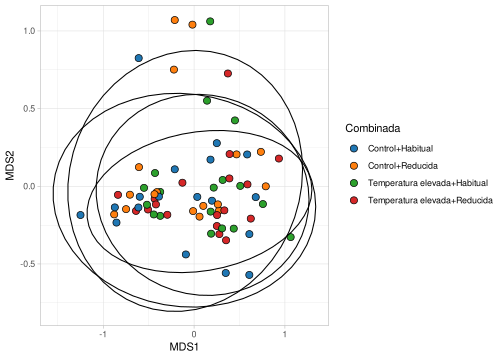
\includegraphics{InformeNeiker_files/figure-pdf/unnamed-chunk-12-3.pdf}

}

\end{figure}



\end{document}
